\documentclass[a4paper,12pt]{report} 

% --------------------------
% CODIFICA E LINGUA
% --------------------------
\usepackage[utf8]{inputenc}   
\usepackage[T1]{fontenc}      
\usepackage[english,italian]{babel}
\usepackage{enumitem}
% --------------------------
% PACCHETTI MATEMATICI
% --------------------------
\usepackage{amsmath, amssymb}
\usepackage{algorithm2e}
\usepackage[margin=2cm]{geometry}
% --------------------------
%q GESTIONE LINK E RIFERIMENTI
% --------------------------
\usepackage{hyperref}         
\hypersetup{
    colorlinks=true,
    linkcolor=blue,
    urlcolor=blue,
    pdftitle={Appunti di Reti e Informatica},
    pdfauthor={},
    pdfpagemode=FullScreen,
}

% --------------------------
% LISTE, BOX, E AMBIENTI
% --------------------------
\usepackage{enumitem}         
\usepackage{tcolorbox}     
\usepackage{xifthen} % per \ifstrempty
\tcbuselibrary{most} % per opzioni avanzate (es. box colorati, notebox, esempiobox)
\usepackage{tikz}

% --------------------------
% GRAFICA E IMMAGINI
% --------------------------
\usepackage{graphicx}
\usepackage{float} % per [H] nelle figure
\usepackage{caption} % per \captionof fuori da table/figure

% --------------------------
% TABELLE
% --------------------------
\usepackage{array}
\usepackage{tabularx}
\usepackage{booktabs} % per tabelle più eleganti (no linee verticali)
\usepackage{longtable}
\usepackage{ltablex}
\usepackage{multirow}
\keepXColumns

% --------------------------
% IMPOSTAZIONI PERSONALIZZATE (facoltative)
% --------------------------
\renewcommand{\arraystretch}{1.2} % più spazio tra le righe delle tabelle
\setlength{\parindent}{0pt} % niente indentazione all'inizio dei paragrafi
\setlist[itemize]{noitemsep, topsep=4pt}
\setlist[enumerate]{noitemsep, topsep=4pt}



% =========================================================
% Box definizione (titolo personalizzabile)
\newtcolorbox{defbox}[2][]{%
  colback=green!10,
  colframe=green!65!black,
  title={Definizione\ifstrempty{#2}{}{ -- #2}},
  #1
}

% Box nota (titolo personalizzabile)
\newtcolorbox{notebox}[2][]{%
  colback=yellow!10,
  colframe=yellow!60!black,
  title={Nota\ifstrempty{#2}{}{ -- #2}},
  #1
}

% Box esempio (titolo personalizzabile)
\newtcolorbox{esempiobox}[2][]{%
  colback=blue!10,
  colframe=blue!65!black,
  title={Esempio\ifstrempty{#2}{}{ -- #2}},
  #1
}


% =========================================================

\title{Reti di Calcolatori  (Modulo I) \\ Capitoli 1 e 2: Introduzione reti di calcolatori e conversioni tra basi}     
\author{Luca Argentino}       
\date{2025 - 2026}

\begin{document}              
\maketitle                    
\tableofcontents              
\newpage                      

% =========================================================
\chapter{Introduzione alle Reti di Calcolatori}

\section{Cos’è una rete di calcolatori?}
\begin{defbox}{Rete di calcolatori}
 insieme di dispositivi di calcolo \textbf{autonomi}, (svolgono compiti autonomamente), interconnessi (tramite supporti fisici).
\end{defbox}

\subsection{Non considerate reti di calcolatori}
\begin{itemize}
  \item Reti di comunicazione telefonica
  \item Reti di distribuzione televisiva 
\end{itemize}
(telefoni, televisioni non sono dispositivi autonomi)

\subsection{Motivazioni allo sviluppo}
\begin{enumerate}
  \item \textbf{Supporto comunicazione tra utenti}: nascono servizi di comunicazione (es. Gmail, WWW, IoT).
  \item \textbf{Comunicazione tra calcolatori}: 
  \begin{itemize}
    \item Condivisione di informazioni(pagine web, data base),dispositivi(stampanti) e risorse(supporti di memorizzazione)
    \item Accesso a calcolatori remoti
    \item Esecuzione calcoli in maniera distribuita
  \end{itemize}
\end{enumerate}

\begin{figure}[H] % H = Here (forza la posizione)
\centering
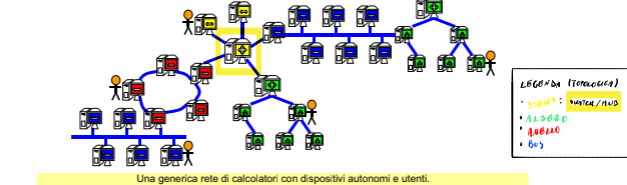
\includegraphics[width=1\linewidth]{foto reti di calcolatori/rete di calcolatori.png}
\end{figure}


\section{Classificazione delle reti in base all' area geografica}
\begin{description}[leftmargin=2cm]

  \item[PAN (Personal Area Network):] collega dispositivi vicini. \\
  \textbf{Esempio:} dispositivi in una stanza/corpo. \\
  \textbf{Finanziate:} da singolo utente.

  \item[LAN (Local Area Network):] connette dispositivi nello stesso edificio/laboratorio. \\
  \textbf{Esempio:} dispositivi in un campus o ufficio. \\
  \textbf{Finanziate:} organizzazioni/enti/aziende/università.

  \item[MAN (Metropolitan Area Network):] estensione di decine di chilometri. \\
  \textbf{Esempio:} accesso cablato reti civiche, aree urbane. \\
  \textbf{Finanziate:} provider e gestori di servizi telefonici.

  \item[WAN (Wide Area Network):] copre distanze nazionali / planetarie. \\
  \textbf{Esempio:} reti cablate o in fibra oppure basate su comunicazioni satellitari. \\
  \textbf{Finanziate:} enti internazionali o grossi enti o gestori delle comunicazioni

   \item[Internet: ]
  Rete di reti conformi a regole di comunicazione.
  Protocollo fondamentale: \textbf{TCP/IP}.
  
\end{description}

\newpage
\newpage
\section{Evoluzione e costi delle reti}

Lo sviluppo delle reti di calcolatori, che ha permesso la nascita di Internet, non sarebbe stato possibile senza una distribuzione dei costi di realizzazione e gestione delle infrastrutture tra molteplici entità. 

Storicamente, la prima rete nasce da un esperimento nel 1969, connettendo solo 4 calcolatori di 4 università americane. Da allora la crescita è stata esponenziale: all'inizio del 2003 si contavano oltre 172 milioni di calcolatori connessi (fonte \textit{Internet Software Consortium}), arrivando a stimare oltre 4 miliardi di dispositivi connessi nel 2020. Con l'avvento dell'\textit{Internet of Things} (IoT), si prevede di raggiungere o superare i 60 miliardi di dispositivi connessi.

Per quanto riguarda i costi di realizzazione e mantenimento, le infrastrutture principali ad alte prestazioni per le reti estese (come MAN e WAN) richiedono investimenti economici elevati. Questi sono tipicamente affrontabili solo attraverso la pianificazione e le risorse di consorzi o grandi fornitori di servizi di comunicazione nazionali e multinazionali.

Tuttavia, la maggior percentuale del complesso delle infrastrutture di rete che compongono Internet risulta essere mantenuta e gestita capillarmente da piccoli gestori e piccoli gruppi, con investimenti relativamente modesti per la realizzazione di \textbf{piccole reti locali} (LAN). 

L’integrazione di un insieme molto vasto di reti grandi e, soprattutto, piccole reti locali, eterogenee e distribuite su tutto il pianeta, ha permesso la crescita incrementale, il successo commerciale e l'esplosiva diffusione delle reti su scala globale, realizzando quel concetto di "rete di reti" che è alla base di Internet.

Infine, l'utente delle reti paga tipicamente per i servizi di trasmissione offerti dai provider, con tariffe che possono essere basate sul tempo di collegamento, sulla quantità di dati scambiati, oppure tramite tariffe "tutto incluso" (flat).

\newpage
\newpage
\section{Prestazioni delle reti}
Per ciò che riguarda le prestazioni delle reti di calcolatori, l'utente è principalmente interessato a tre indici fondamentali:

\subsection*{1. Capacità di trasmissione (bit rate)}
\begin{defbox}{}
Misurata in bit/sec (e nei suoi multipli Kbit/s, Mbit/s, Gbit/s): indica la quantità massima di dati digitali che è possibile trasmettere o ricevere in un secondo attraverso il collegamento di rete.
\end{defbox}

\begin{notebox}{\textbf{Attenzione!}}
Nelle offerte commerciali viene solitamente indicato il valore massimo teorico di dati che si possono mandare/ricevere, ma la banda o limite minimo non è quasi mai garantito.
\end{notebox}

\textbf{L'analogia del tubo:} Pensando concettualmente alle reti come a tubi che trasportano bit, la capacità di trasmissione equivale al \textbf{diametro del tubo}.

\subsection*{2. Ritardo del collegamento di rete (Latenza)}
\begin{defbox}{}
Indica il tempo richiesto ai dati per transitare fisicamente dal mittente al destinatario finale. Spesso si utilizza anche la metrica \textbf{RTT (Round Trip Time)}, misurata in millisecondi (ms), che indica invece il ritardo totale di \textbf{andata e ritorno} di un pacchetto (dal client al server e viceversa).
\end{defbox}

Il ritardo è determinato dall'attraversamento di varie tappe intermedie. Le cause principali sono:
\begin{itemize}
    \item \textbf{Distanza fisica} del collegamento.
    \item \textbf{Tempi di gestione dei protocolli} (tempi di elaborazione richiesti ai dispositivi intermedi per applicare le leggi dei processi di comunicazione).
\end{itemize}

\textbf{L'analogia del tubo:} Riprendendo l'esempio precedente, il ritardo equivale alla \textbf{lunghezza del tubo} (il tempo che i bit impiegano ad attraversarlo nella sua interezza).

\begin{notebox}{\textbf{Attenzione!}}
Tra \textbf{capacità di trasmissione} (larghezza di banda) e \textbf{ritardo del collegamento} (latenza) non esiste una metrica più importante in assoluto: la priorità dell'una o dell'altra dipende strettamente dal tipo di applicazione utilizzata.

\begin{itemize}
    \item \textbf{Navigazione Web (Browsing)}
    \begin{itemize}
        \item L'apertura di \textbf{pagine "pesanti"} (ricche di contenuti multimediali) richiede un'\textbf{alta capacità di trasmissione} per scaricare rapidamente la grande mole di dati.
        \item L'apertura di \textbf{pagine "leggere"} (testo o piccoli file) è invece più sensibile a un \textbf{basso ritardo di collegamento}, per ridurre i tempi di reazione del server.
    \end{itemize}
    
    \item \textbf{Posta elettronica (E-mail)}
    \begin{itemize}
        \item Essendo un servizio \textbf{asincrono}, è molto tollerante e non ha requisiti stringenti per nessuna delle due metriche (salvo il caso di grossi allegati, che richiedono più capacità).
    \end{itemize}
    
    \item \textbf{Videogiochi online (Gaming in tempo reale)}
    \begin{itemize}
        \item Necessitano di un \textbf{RTT estremamente basso} (ping). La quantità di dati scambiata è minima, ma è vitale che l'invio dei comandi, la percezione del server e l'invio della "nuova realtà" avvengano istantaneamente per evitare il \textit{lag}.
    \end{itemize}
\end{itemize}
\end{notebox}



\newpage
\subsection*{3. Jitter (Fluttuazione del ritardo)}
\begin{defbox}{}
Indica la \textbf{varianza} (o dispersione/spargimento intorno al valore medio) del ritardo di rete. Misura quanto il ritardo di ricezione oscilla e cambia tra i vari pacchetti di una singola sequenza.
\end{defbox}

% Ti consiglio di ritagliare dalla slide 10 il grafico con i pallini rossi e blu e inserirlo qui:
\begin{figure}[h]
    \centering
    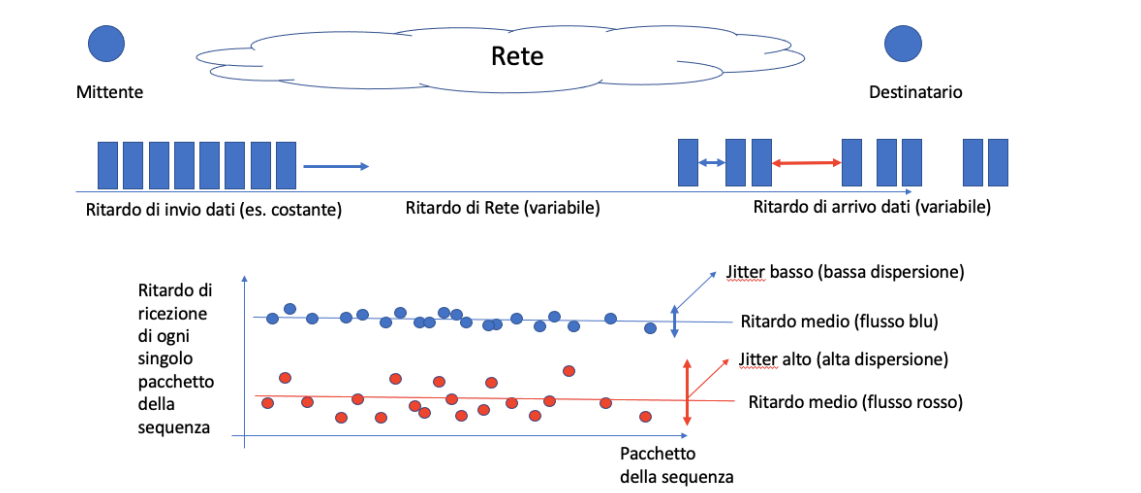
\includegraphics[width=0.9\textwidth]{foto reti di calcolatori/jitter.png}
    \caption{Confronto visivo: un flusso con ritardo medio alto ma Jitter basso (pallini blu) risulta spesso migliore e più facile da gestire rispetto a un flusso apparentemente più veloce ma con Jitter alto e disperso (pallini rossi).}
\end{figure}

A seconda dell'applicazione, il Jitter ha impatti e soluzioni differenti:
\begin{itemize}
    \item \textbf{Videocall (Comunicazione interattiva):} Le applicazioni VoIP non possono attendere troppo, quindi i pacchetti in forte ritardo a causa del jitter vengono ignorati o persi, causando i tipici "scatti" o blocchi nell'audio/video.
    \item \textbf{Streaming (Media on-demand):} Richiede un flusso assolutamente costante. Il jitter della rete viene assorbito e annullato interponendo un \textbf{buffer di memoria} locale prima della riproduzione.
\end{itemize}


\subsubsection*{Il ruolo del Buffer}
Il buffer agisce come un "serbatoio" che si riempie in modo irregolare (dalla rete) ma si svuota in modo costante (verso lo schermo dell'utente).

\begin{itemize}
    \item \textbf{Vantaggi del buffer}:
        \begin{itemize}
          \item Assorbe le fluttuazioni di rete (il jitter), garantendo una riproduzione continua e fluida dei dati.
          \item Fondamentale ed estremamente efficace per lo streaming video o audio non interattivo (es. Netflix).
        \end{itemize}
    
    \item \textbf{Svantaggi del buffer}:
        \begin{itemize}
          \item Introduce un ritardo di attesa artificiale ($\Delta t$), poiché bisogna aspettare che il buffer si riempia parzialmente prima di poter mostrare l'evento a schermo.
          \item Inutilizzabile per i sistemi \textit{real-time} interattivi dove il ritardo distruggerebbe l'esperienza utente.
        \end{itemize}
\end{itemize}

\begin{esempiobox}{Jitter: Skype vs Netflix}
Per capire l'impatto del Jitter, ricordiamo che un \textbf{Jitter basso è sempre la condizione ideale}. La differenza sta nella tolleranza delle applicazioni all'instabilità della rete:

\begin{itemize}
    \item \textbf{Scenario 1: Videocall su Skype (Bassa Tolleranza)}
    \begin{itemize}
        \item \textit{Cosa succede con Jitter Basso:} I pacchetti audio/video arrivano con un ritmo costante. La conversazione è fluida e naturale.
        \item \textit{Cosa succede con Jitter Alto:} I pacchetti arrivano a "singhiozzo". La voce diventa metallica, si formano silenzi imbarazzanti seguiti da parole parlate tutte d'un fiato, oppure cade la linea. Il sistema non ha il tempo di aspettare i pacchetti in ritardo.
    \end{itemize}
    
    \vspace{0.3cm}
    
    \item \textbf{Scenario 2: Film su Netflix (Alta Tolleranza)}
    \begin{itemize}
        \item \textit{Cosa succede con Jitter Basso:} Il film inizia quasi subito e procede senza intoppi, il buffer si riempie in modo omogeneo.
        \item \textit{Cosa succede con Jitter Alto:} Il film si vede comunque bene! Questo accade non perché il Jitter alto sia un vantaggio, ma perché Netflix costringe il tuo dispositivo ad aspettare qualche secondo prima di far partire il video (\textbf{Buffer}). Il serbatoio di memoria assorbe il "singhiozzo" dei pacchetti, nascondendo il problema della rete ai tuoi occhi.
    \end{itemize}
\end{itemize}
\end{esempiobox}



\newpage
\section{Componenti di una Rete}
Per connettere un calcolatore alla rete è richiesto un insieme minimo di componenti HW e SW:
\begin{enumerate}
  \item \textbf{Dispositivi o schede di rete:} 
  \begin{itemize}
      \item dispositivi hardware collegati al calcolatore
      \item codificano, trasmettono, ricevono, decodificano dati dal calcolatore alla rete e viceversa
      \item sono gestiti da software del sistema operativo come i \textbf{driver} che fanno da collante tra macchina e sistema software (senza di essi le schede di rete non verrebero riconosciute)
  \end{itemize}
  
  \item \textbf{Mezzi di trasmissione:} supporti fisici per trasmissione dei segnali: cavi elettrici, fibra ottica, wireless.
  
  \item \textbf{Connettori di rete:} interfacce standard (es. Ethernet RJ45) presenti sul dispositivo di rete per connettersi al mezzo di trasmissione della rete.
  \item \textbf{Protocolli di rete:} insiemi di regole implementate sottoforma di software per garantire compatibilità e gestione della comunicazione(TCP/IP).
\end{enumerate}

\begin{figure}[H] % H = Here (forza la posizione)
\centering
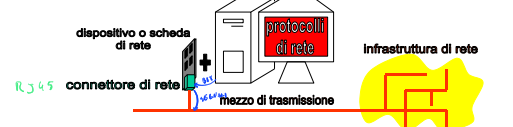
\includegraphics[width=1\linewidth]{foto reti di calcolatori/componenti rete di calcolatori.png}
\end{figure}

\subsection{Dispositivi o schede di rete}
Le \textbf{schede di rete} (NIC, Network Interface Card) sono dispositivi hardware che permettono al calcolatore di comunicare con la rete.  

Ogni scheda di rete possiede un indirizzo univoco chiamato \textbf{indirizzo MAC} (Media Access Control), usato per identificare la scheda a livello di collegamento, così da limitare le collisioni, in quanto viene specificato il mittente e il destinatario 

\begin{itemize}
  \item Convertono i dati digitali del calcolatore in segnali elettrici, ottici o radio.
  \item Gestiscono la \textbf{trasmissione} (dal calcolatore al mezzo di trasmissione) e \textbf{ricezione} (dal mezzo di trasmissione al calcolatore) dei frame sulla rete.
  \item Interagiscono con il sistema operativo tramite \textbf{driver}, che fungono da interfaccia software per l’hardware di rete.
  \item Il tipo della scheda di rete viene identificato a seconda del mezzo trasmissivo, e soprattutto a seconda dei protocolli di comunicazione utilizzati per la codifica, e per la trasmissione dei dati in rete (es: Ethernet, Wi-Fi, Bluetooth)
  \item è dotata di  \begin{enumerate}
      \item un \textbf{interfaccia di collegamento} al calcolatore 
      \item un \textbf{connettore} di rete, che pone direttamente in contatto la scheda di rete con il mezzo di trasmissione per l’invio e ricezione dei segnali in rete.
  \end{enumerate}
\end{itemize}

\begin{figure}[H]
\centering
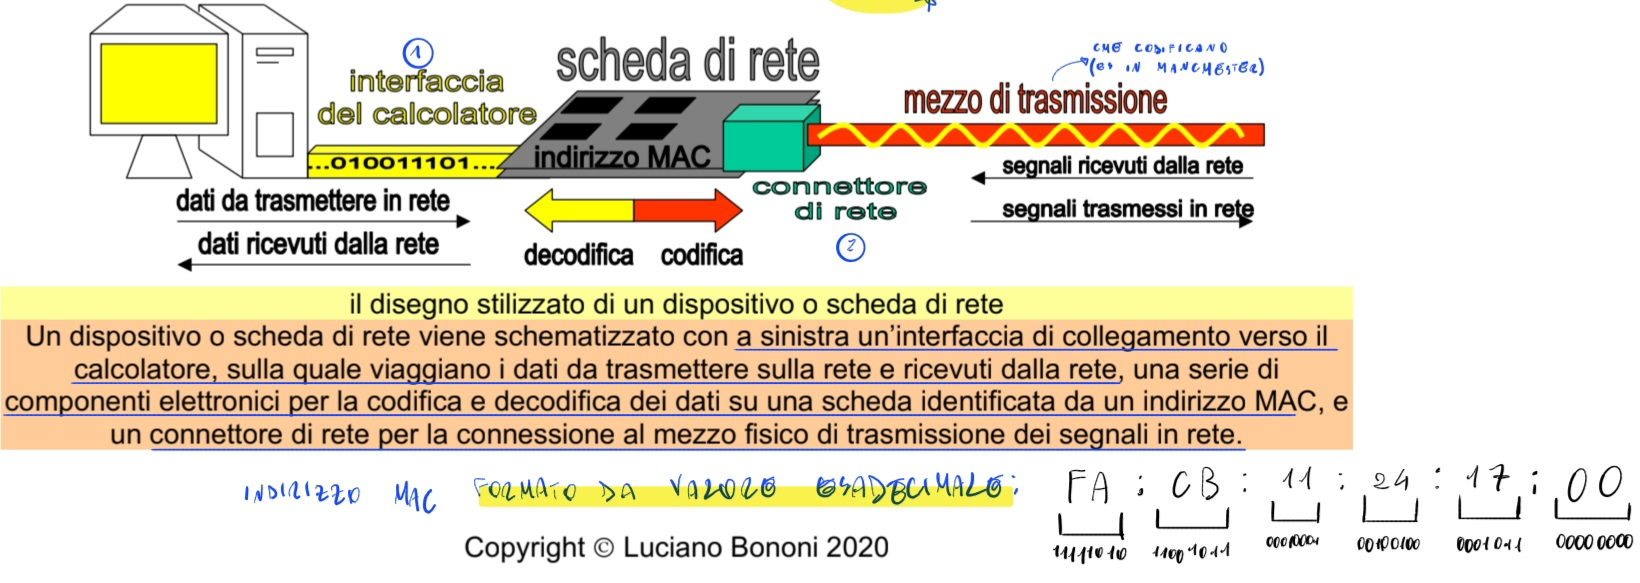
\includegraphics[width=1\linewidth]{foto reti di calcolatori/scheda_rete.jpg}
\caption{Esempio di scheda di rete}
\end{figure}




\newpage
\section {Infrastrutture e Collegamenti di Rete}
Un collegamento o connessione fisica di rete è fornita da un mezzo di trasmissione(cavi,fibra oppure wifi)

\begin{defbox}{Infrastruttura di rete}
    
Un’\textbf{infrastruttura di rete} rappresenta l’insieme dei collegamenti o connessioni fisiche esistenti tra tutti i dispositivi di una rete.
\end{defbox}

La comunicazione tra una coppia qualsiasi di calcolatori in rete, detti nodi (oppure host) della rete, è possibile se esiste un collegamento diretto tra i nodi, oppure se esiste una sequenza di collegamenti, detta cammino, che permetta la comunicazione dei segnali passando per eventuali nodi e collegamenti intermedi.

Sono possibili diverse classi di strutture di connessione della rete.

\subsection{Classi di infrastruttura}
\begin{enumerate}
  \item \textbf{Punto a punto (send <-> recive)}: connessione diretta tra due calcolatori.
  \item \textbf{Connessioni multiple}: 
  \begin{itemize}
    \item \textbf{completamente connessa (cammini rindondanti)} ogni dispositivo collegato a tutti gli altri. 
      \begin{itemize}
        \item Vantaggi: tolleranza ai guasti e sempre cammino diretto esistente (esistono diverse strade alternative) 
        \item Svantaggi: costosa e complessa
      \end{itemize}
    \item \textbf{parzialmente connessa:} ogni calcolatore(nodo) connesso solo ad alcuni. 
      \begin{itemize}
        \item Vantaggi: costo ridotto, facile da realizzare, densità di protocollo bassa
        \item Svantaggi: fragilità se cade un nodo
      \end{itemize}
    \item \textbf{partizione di rete:} nodi in sottoreti isolate. 
      \begin{itemize}
        \item Vantaggi: sicurezza, controllo accessi
        \item Svantaggi: rete divisa in isole
      \end{itemize}
  \end{itemize}
\end{enumerate}

\textbf{obiettivo}: trovare bilanciamento tra robustezza, costo e velocità

\begin{figure}[H] % H = Here (forza la posizione)
\centering
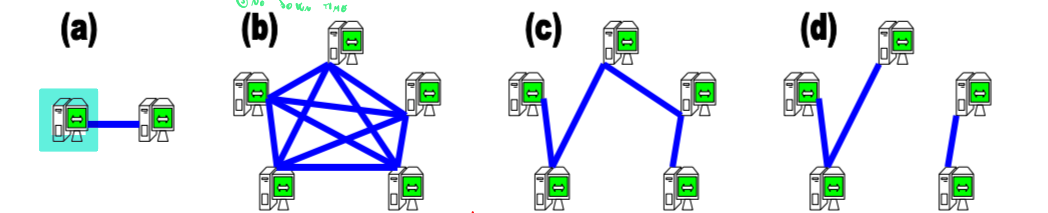
\includegraphics[width=1\linewidth]{foto reti di calcolatori/Classi di infrastruttura.png}
\caption{Classi di infrastrutture}
\end{figure}

\newpage
\section{Topologie di rete}
Le infrastrutture di rete possono essere organizzate secondo diverse \textbf{topologie}, ossia schemi di connessione tra nodi:



\subsection{Principali topologie}
\begin{enumerate}[label=\alph*)]
  \item \textbf{Anello (Ring):} ogni nodo connesso a due vicini e può comunicare con ogni altro componente inviando i segnali attraverso la sequenza di connessioni in senso orario o antiorario.
  \item \textbf{Stella (Star):} tutti i nodi connessi a un nodo centrale (hub/switch).Ogni componente periferico può comunicare con ogni altro componente periferico passando attraverso il componente centrale.
  \item \textbf{Bus:} tutti i nodi condividono un unico canale. Basso costo ma alta possibilità di collisioni (in quanto va gestito benel'accesso al bus).
  \item \textbf{Albero (Tree):} struttura gerarchica con nodi principali e secondari.
 
\end{enumerate}

\begin{figure}[H]
\centering
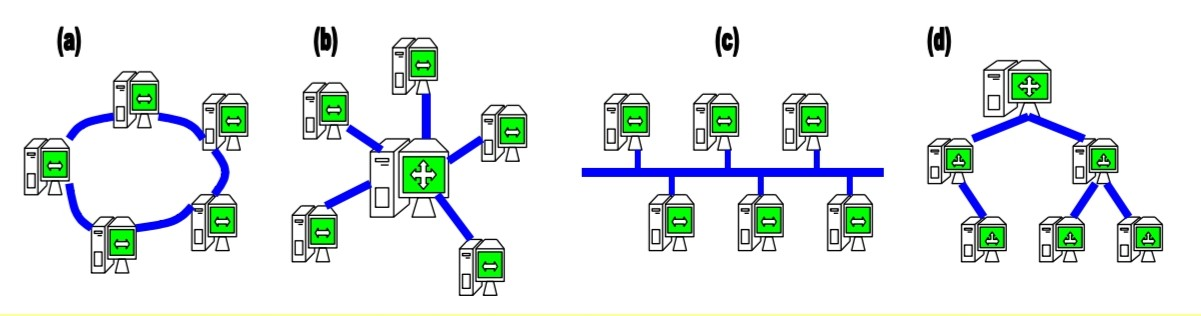
\includegraphics[width=\linewidth]{foto reti di calcolatori/topologie.jpg}
\caption{Esempi di topologie: anello, stella, bus, albero.}
\end{figure}

\begin{notebox}{}
Le reti reali spesso adottano \textbf{topologie ibride}, combinando più modelli (es. stella su bus o maglia parziale).
\end{notebox}


\newpage
\subsection{Confronto tra topologie}
\noindent
Di seguito vengono confrontate le principali \textbf{topologie di rete}, evidenziandone i vantaggi e gli svantaggi in termini di affidabilità, tolleranza ai guasti e connettività minima.

\bigskip

\textbf{1. Topologia ad Anello (Ring)}
\begin{itemize}[leftmargin=*]
  \item \textbf{Vantaggi:}
  \begin{itemize}
    \item \textbf{Trasmissione ordinata e deterministica:} un solo nodo trasmette per volta, azzerando il rischio di collisioni.
    \item \textbf{Latenza prevedibile:} ideale per traffico con vincoli temporali rigidi (es. reti Token Ring).
    \item \textbf{Acknowledgment (Riscontro) implicito:} un pacchetto che, dopo la consegna, completa il giro e ritorna al mittente nello stesso verso, funge da conferma automatica dell'avvenuta ricezione.
    \item \textbf{Tolleranza ai guasti (solo Anello Doppio):} la presenza di un anello secondario introduce ridondanza. Offre una tolleranza parziale garantendo l'\textbf{autoriparazione} in caso di un singolo guasto (il traffico torna indietro chiudendo l'anello a forma di "C").
    \item \textbf{Efficienza del percorso (solo Anello Doppio):} i dati possono viaggiare in entrambe le direzioni scegliendo la via più breve. Il percorso massimo (\textit{path} peggiore) si dimezza a $n/2$ salti.
  \end{itemize}
  
  \item \textbf{Svantaggi:}
  \begin{itemize}
    \item \textbf{Vulnerabilità (Anello Singolo):} essendo una rete \textit{minimamente connessa}, non offre alcuna ridondanza. Il guasto di un singolo nodo o di un singolo collegamento interrompe l'intera rete.
    \item \textbf{Percorso lungo (Anello Singolo):} poiché i dati viaggiano in un'unica direzione, il percorso peggiore per raggiungere un nodo richiede $n-1$ salti (dove $n$ è il numero totale di dispositivi).
    \item \textbf{Scarsa scalabilità:} in anelli molto grandi, la latenza di attraversamento cresce in modo lineare con l'aggiunta di nuovi nodi.
    \item \textbf{Costi e complessità:} l'implementazione del doppio anello, necessaria per risolvere i problemi di affidabilità, aumenta notevolmente i costi hardware e la complessità di gestione dell'infrastruttura.
  \end{itemize}
\end{itemize}

\vspace{1cm}
\textbf{2. Topologia a Stella (Star)}
\begin{itemize}[leftmargin=*]
  \item \textbf{Vantaggi:}
  \begin{itemize}
    \item \textbf{Standard di fatto:} è l'architettura in assoluto più utilizzata per le moderne reti locali (LAN) Ethernet.
    \item \textbf{Isolamento dei guasti periferici:} la rottura di un cavo o il malfunzionamento di un singolo nodo periferico isola solamente quel dispositivo, senza compromettere il funzionamento del resto della rete.
    \item \textbf{Flessibilità e scalabilità:} aggiungere, rimuovere o individuare nodi difettosi è un'operazione estremamente semplice a livello di gestione e manutenzione.
    \item \textbf{Alta efficienza (se basata su Switch):} se il nodo centrale è uno \textbf{Switch} (livello 2 - MAC/LLC), questo inoltra i pacchetti solo alla porta del destinatario. Ciò permette comunicazioni simultanee punto-a-punto, separando i domini di collisione e azzerando di fatto il rischio di scontri tra pacchetti.
  \end{itemize}

  \newpage
  \item \textbf{Svantaggi:}
  \begin{itemize}
    \item \textbf{Single Point of Failure (Punto critico di guasto):} la dipendenza dal nodo centrale è totale. Se il centro stella (Hub o Switch) si guasta o si spegne, l'intera comunicazione di rete si paralizza istantaneamente.
    \item \textbf{Problemi di congestione (se basata su Hub):} se realizzata con un \textbf{Hub} (livello 1 - Fisico), il dispositivo si limita a replicare il segnale elettrico su tutte le porte. L'intera rete diventa un unico grande \textbf{dominio di collisione}\footnote{Collision domain: Un'area logica della rete in cui i segnali trasmessi contemporaneamente da due o più dispositivi si sovrappongono e collidono, distruggendosi a vicenda e causando ritardi (\textit{jammer}).}, le cui prestazioni crollano drasticamente all'aumentare degli utenti attivi.
    \item \textbf{Vincoli di cablaggio:} rispetto a topologie come il bus o l'anello, richiede un quantitativo di cavo nettamente superiore, poiché ogni singolo dispositivo necessita di una linea fisica dedicata per raggiungere il nodo centrale.
    \item \textbf{Connettività minima:} pur essendo molto robusta sui rami periferici, non offre ridondanza di percorso. Esiste esattamente un solo cammino (path) per raggiungere ciascun nodo dalla base centrale.
  \end{itemize}
\end{itemize}

\vspace{1cm}
\textbf{3. Topologia a Bus}
\begin{itemize}[leftmargin=*]
  \item \textbf{Vantaggi:}
  \begin{itemize}
    \item \textbf{Semplicità ed economicità:} richiede una quantità minima di cablaggio, risultando l'architettura più economica e facile da implementare per reti locali di piccolissime dimensioni.
    \item \textbf{Assenza di un nodo centrale:} Si elimina la dipendenza hardware da un singolo dispositivo di smistamento.
    \item \textbf{Espandibilità iniziale:} è molto semplice aggiungere nuovi dispositivi collegandoli direttamente al cavo dorsale condiviso (\textit{backbone}).
  \end{itemize}
  
  \item \textbf{Svantaggi:}
  \begin{itemize}
    \item \textbf{Mezzo condiviso (Broadcast):} tutti i dispositivi condividono lo stesso canale fisico. Solo un \textit{host} può trasmettere per volta, introducendo l'esigenza di regole rigide per l'accesso al mezzo.
    \item \textbf{Dominio di collisione unico:} l'intera rete è un unico \textbf{collision domain}. Se due nodi trasmettono contemporaneamente, i segnali si scontrano.
    \item \textbf{Effetto Jamming (Interferenza):} in caso di collisione, i segnali elettrici si sovrappongono corrompendosi a vicenda (\textit{jammer}). L'informazione viene distrutta e i nodi devono interrompere la trasmissione per riprovare più tardi.
    \item \textbf{Vulnerabilità della dorsale:} sebbene non ci sia un nodo centrale, la rottura o il malfunzionamento del singolo cavo principale interrompe l'intera rete o la frammenta in partizioni isolate.
    \item \textbf{Tolleranza ai guasti assente:} la rete è \textit{minimamente connessa}; non esiste alcun percorso alternativo in caso di guasto.
  \end{itemize}
\end{itemize}
\newpage
\textbf{4. Topologia ad Albero (Tree)}
\begin{itemize}[leftmargin=*]
  \item \textbf{Vantaggi:}
  \begin{itemize}
    \item \textbf{Struttura gerarchica e modulare:} organizza i nodi in livelli logici analoghi a un albero genealogico (padre, figlio, nipote), rendendo la gestione e la manutenzione della rete molto ordinata.
    \item \textbf{Scalabilità per grandi reti:} permette di combinare facilmente più topologie (es. collegando tra loro i centri di diverse reti a stella), risultando ideale per reti LAN ampie o distribuite in più uffici/edifici.
    \item \textbf{Segmentazione del traffico:} la gerarchia facilita la divisione logica della rete, permettendo di controllare e isolare il traffico per dipartimenti o gruppi di lavoro.
  \end{itemize}

  \item \textbf{Svantaggi:}
  \begin{itemize}
    \item \textbf{Effetto a cascata dei guasti:} il malfunzionamento di un nodo di livello superiore (il "padre") isola istantaneamente tutti i rami sottostanti (i "figli" e "nipoti"), creando \textbf{partizioni di rete}.
    \item \textbf{Connettività minima:} non esistono collegamenti trasversali tra rami diversi. C'è esattamente un solo percorso disponibile per collegare un nodo figlio a qualsiasi altro nodo.
    \item \textbf{Tolleranza ai guasti limitata:} in assenza di percorsi alternativi e di ridondanza, la rottura di un collegamento gerarchico compromette in modo irreversibile la comunicazione per quell'intera sezione.
  \end{itemize}
\end{itemize}
\vspace{1cm}

% =========================================================
\section{Mezzi fisici di trasmissione}

\begin{itemize}

  \item \textbf{Cavi di materiale conduttore (Twisted Pair, Coassiale):}
  \begin{itemize}
    \item \textbf{Vantaggi:}
      \begin{itemize}
        \item Economici e facili da installare.
        \item Diffusi nelle reti locali (LAN).
        \item Buon rapporto tra costo e prestazioni (fino a 1--2 Gbit/sec).
      \end{itemize}
    \item \textbf{Svantaggi:}
      \begin{itemize}
        \item Sensibili alle interferenze elettromagnetiche.
        \item Distanza di trasmissione limitata.
      \end{itemize}
  \end{itemize}

  \item \textbf{Fibra ottica:}
  \begin{itemize}
    \item \textbf{Vantaggi:}
      \begin{itemize}
        \item Altissima capacità di trasmissione (fino a diverse migliaia di Gbit/sec).
        \item Immunità ai disturbi elettromagnetici.
        \item Distanze di trasmissione molto elevate.
      \end{itemize}
    \item \textbf{Svantaggi:}
      \begin{itemize}
        \item Costo più elevato rispetto ai cavi in rame.
        \item Maggiore fragilità meccanica.
      \end{itemize}
  \end{itemize}

  \item \textbf{Wireless (approfondiremo nel Cap 7):}
  \begin{itemize}
    \item \textbf{Vantaggi:}
      \begin{itemize}
        \item Grande flessibilità e mobilità.
        \item Nessun cablaggio necessario.
      \end{itemize}
    \item \textbf{Svantaggi:}
      \begin{itemize}
        \item Minore sicurezza dei dati trasmessi.
        \item Maggiore suscettibilità a interferenze e ostacoli fisici.
        \item Prestazioni inferiori (da 1 a 54 Mbit/sec).
      \end{itemize}
  \end{itemize}

\end{itemize}

\begin{figure}[H]
\centering
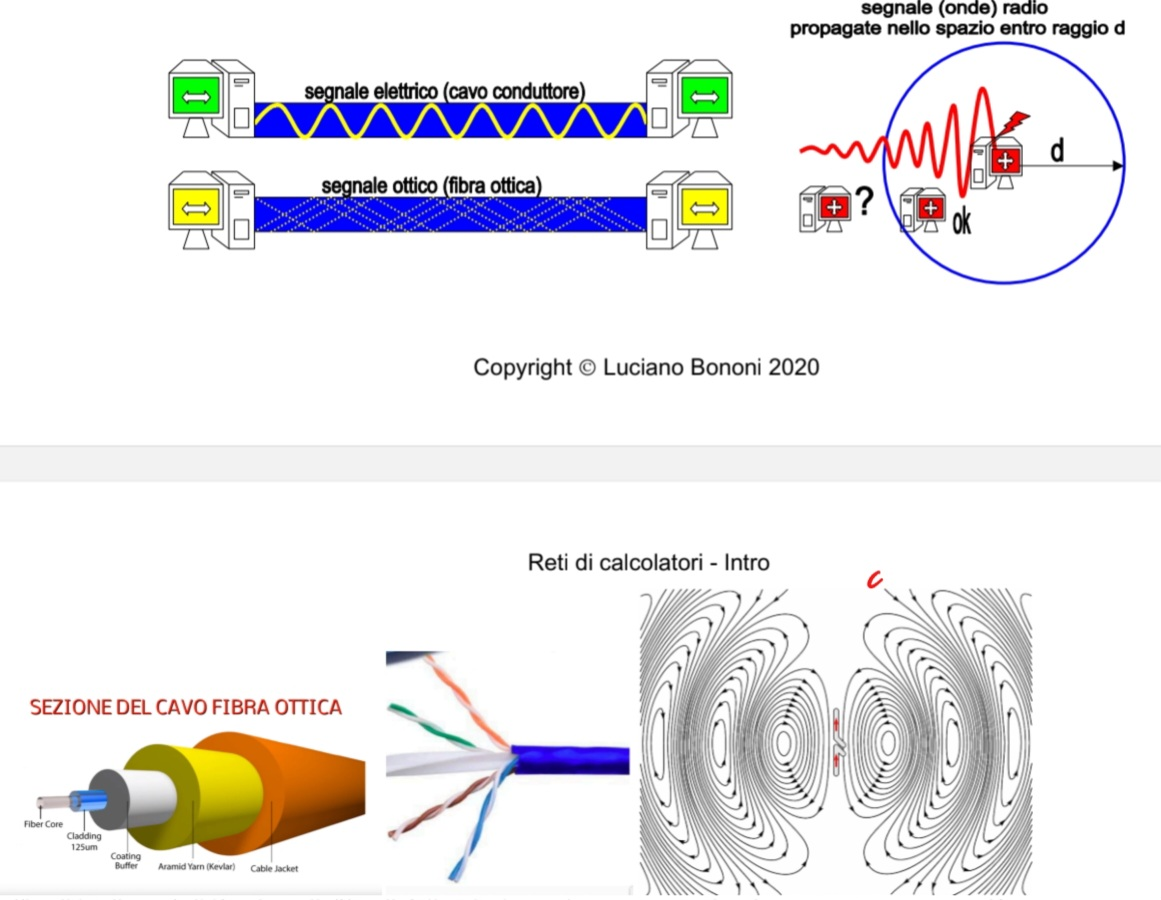
\includegraphics[width=0.8\linewidth]{foto reti di calcolatori/mezzi_trasmissivi.jpg}
\caption{Principali mezzi fisici di trasmissione: cavo conduttore, fibra e wireless.}
\end{figure}

\newpage
\section{Codifica di linea:(APPROFONDIMENTO)}

La \textbf{codifica di linea} trasforma i dati digitali in un segnale fisico trasmissibile (su rame, fibra o radio).  
Una buona codifica deve:
\begin{itemize}
    \item ridurre gli errori di trasmissione;
    \item mantenere la sincronizzazione tra trasmettitore e ricevitore;
    \item ottimizzare l’uso della banda;
    \item limitare la componente continua (DC\footnote{La \textbf{componente continua} (DC, \textit{Direct Current}) rappresenta il valore medio di un segnale nel tempo. In termini pratici, indica l'offset (lo spostamento fisso) rispetto allo zero attorno al quale il segnale oscilla. Costituisce la parte statica del segnale, ovvero la sua componente a frequenza zero.}).
\end{itemize}

\textbf{Clock e sincronizzazione:}  
Il \textit{clock} indica quando campionare i bit.  
Se il segnale non presenta transizioni regolari (es. sequenze di 1 o 0 in NRZ), il ricevitore può perdere la sincronizzazione.  
Alcune codifiche (es. Manchester, 8B/10B) introducono transizioni controllate per consentire di \textbf{ricostruire il clock} dal segnale ricevuto.

\begin{figure}[H]
\centering
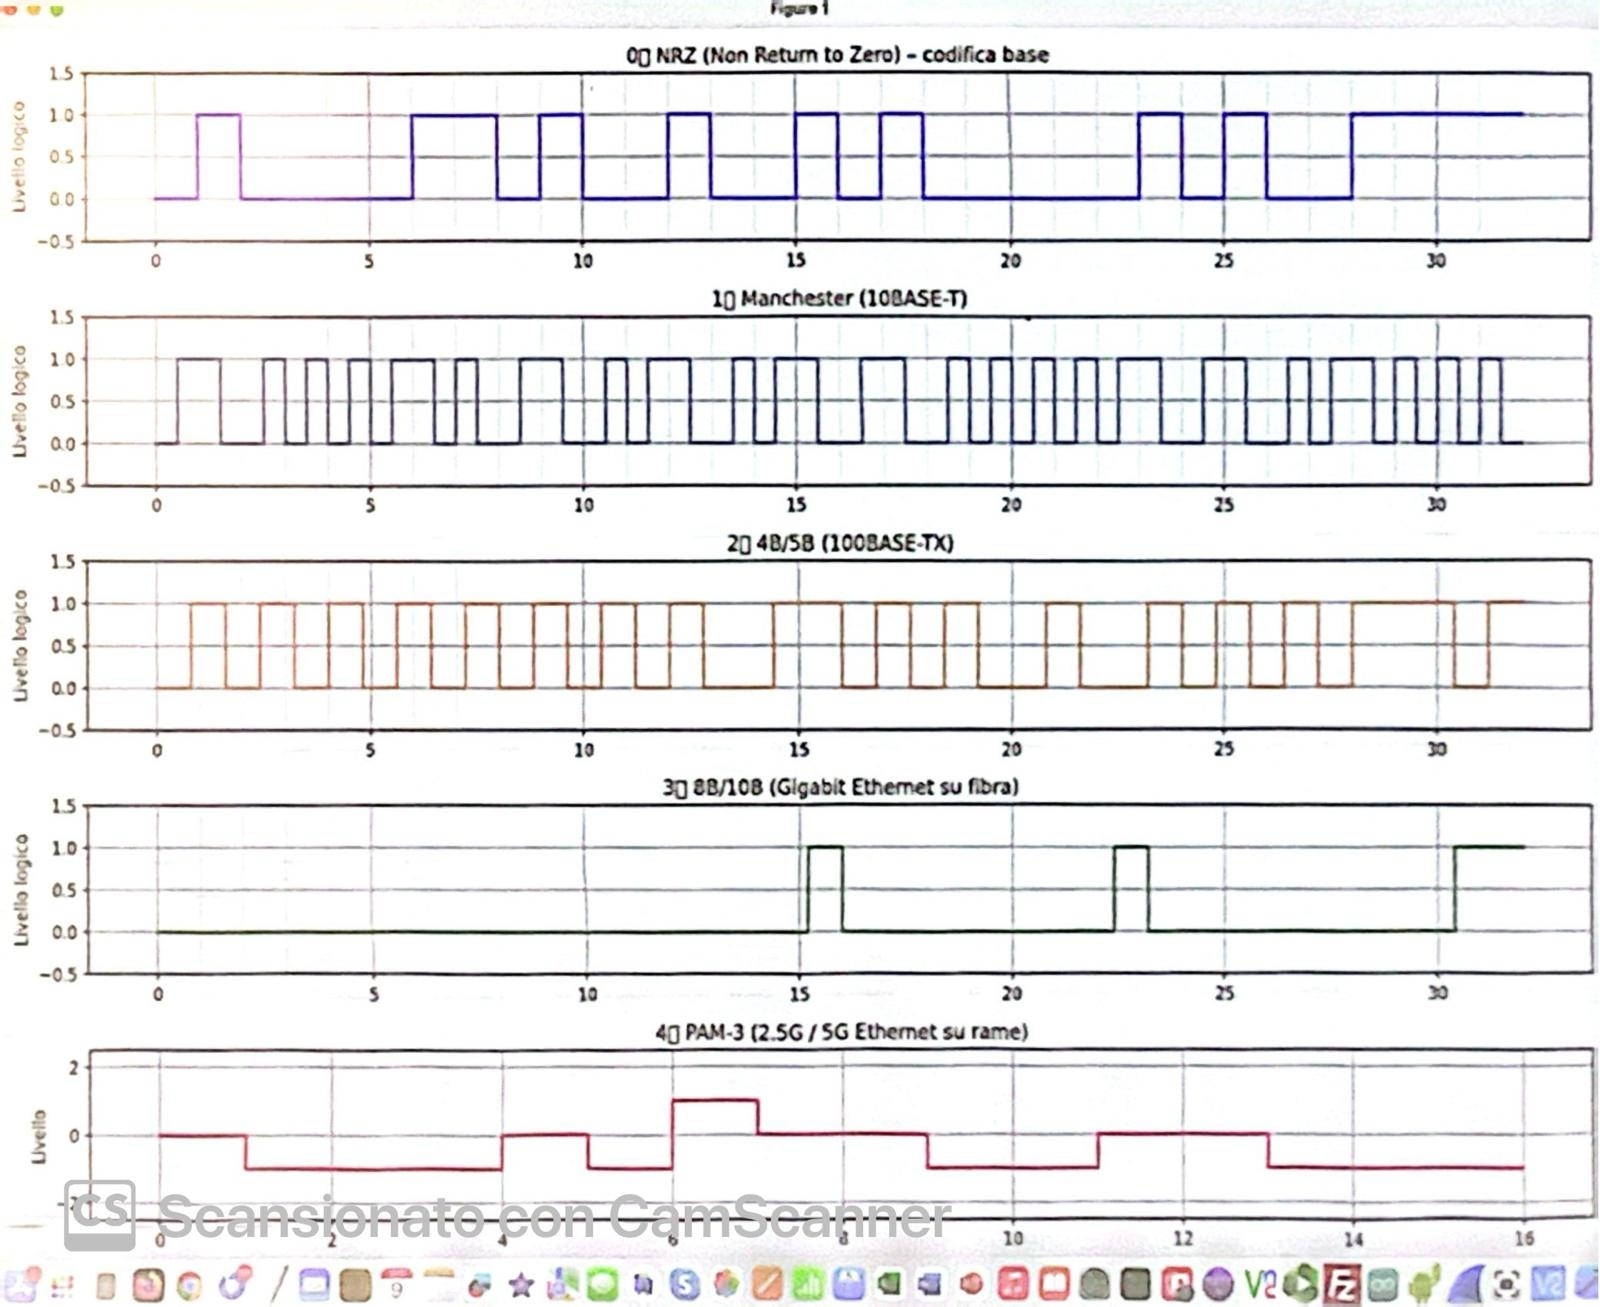
\includegraphics[width=0.9\linewidth]{foto reti di calcolatori/codifiche.jpg}
\end{figure}

%------------------------------------------------
\subsubsection{NRZ (Non Return to Zero)}

Ogni bit è rappresentato da un livello costante di tensione per tutta la sua durata:
\begin{itemize}
    \item \textbf{NRZ:} 1 = livello alto (es. +V), 0 = livello basso (es. -V oppure 0).
\end{itemize}

\textbf{Vantaggi:}
\begin{itemize}
    \item \textbf{Semplice da implementare:} la circuiteria necessaria è basilare, essendoci una corrispondenza diretta e fissa tra il valore del bit e il voltaggio fisico, senza dover gestire salti intermedi durante il tempo di bit.
    \item \textbf{Richiede poca banda:} poiché la tensione cambia solo quando il bit successivo è diverso dal precedente, il numero di transizioni sul cavo è minimo. Meno salti di tensione significano una frequenza del segnale più bassa e, quindi, minor occupazione di banda.
\end{itemize}

\textbf{Svantaggi:}
\begin{itemize}
    \item \textbf{Perdita di sincronizzazione:} il ricevitore usa i "salti" di tensione del segnale in arrivo per mantenere sincronizzato il proprio orologio interno (clock). Se arriva una lunga sequenza di bit uguali (es. 00000000...), il segnale rimane piatto. Senza salti, il ricevitore perde il ritmo e rischia di non capire esattamente quanti zeri consecutivi ha appena letto.
    \item \textbf{Presenza di componente continua (DC)}\ una lunga serie di uni (tutta tensione alta) o di zeri (tutta tensione bassa) sposta nettamente il valore medio del segnale lontano dallo zero. Questo accumulo di energia "statica" non può attraversare alcuni componenti fisici di rete (come i trasformatori di isolamento) e rischia di distorcere gravemente il segnale.
\end{itemize}

%-------------------------------------------------
\subsubsection{Manchester}

Ogni bit è caratterizzato da una \textbf{transizione garantita a metà del tempo di bit}:
\begin{itemize}
    \item \textbf{1} $\rightarrow$ transizione da livello basso a livello alto.
    \item \textbf{0} $\rightarrow$ transizione da livello alto a livello basso (o viceversa, a seconda della convenzione utilizzata).
\end{itemize}

\textbf{Vantaggi:}
\begin{itemize}
    \item \textbf{Sincronizzazione automatica (Self-clocking):} a differenza dell'NRZ, avendo un "salto" di tensione sempre garantito esattamente a metà di \textit{ogni singolo bit}, il ricevitore ha un riferimento temporale continuo. Non perde mai il ritmo (clock), nemmeno se riceve una sequenza infinita di zeri o di uni.
    \item \textbf{Assenza di componente continua (DC):} poiché ogni singolo bit trascorre obbligatoriamente metà del suo tempo a livello alto e metà a livello basso, la media della tensione sul cavo si annulla perfettamente. Questo azzera i problemi di accumulo di energia statica e di distorsione visti nell'NRZ.
\end{itemize}

\textbf{Svantaggi:}
\begin{itemize}
    \item \textbf{Banda occupata doppia (Bassa efficienza):} per garantire quel salto centrale a ogni bit, il segnale Manchester compie fino al doppio delle transizioni di tensione rispetto all'NRZ (spesso deve fare un salto aggiuntivo tra un bit e l'altro per "riposizionarsi"). Cambiando tensione più velocemente, la frequenza del segnale raddoppia: a parità di bit trasmessi, il Manchester divora il doppio della larghezza di banda fisica del cavo.
\end{itemize}

\textbf{Utilizzo:} \textbf{Ethernet 10BASE-T} (il classico standard LAN su doppino in rame a 10 Mbit/s).
%-------------------------------------------------
\subsubsection{Codifica 4B/5B}

Ogni gruppo di 4 bit è codificato in 5 bit, scegliendo combinazioni che garantiscono transizioni regolari.  
È spesso abbinata a \textbf{NRZ-I} per la trasmissione fisica.

\textbf{Vantaggi:}
\begin{itemize}
    \item Migliore sincronizzazione rispetto a NRZ.
    \item Nessuna lunga sequenza di zeri.
\end{itemize}

\textbf{Utilizzo:} Fast Ethernet (100Base-TX).

%-------------------------------------------------
\subsubsection{Codifica 8B/ (Gigabit Ethernet su fibra)}

Ogni byte (8 bit) viene codificato in 10 bit, garantendo:
\begin{itemize}
    \item bilanciamento tra 1 e 0 (\textit{disparity});
    \item transizioni regolari per un facile recupero del clock.
\end{itemize}

\textbf{Vantaggi:}
\begin{itemize}
    \item Sincronizzazione stabile anche ad alte velocità.
    \item Assenza di componente continua.
\end{itemize}

\textbf{Utilizzo:} Gigabit Ethernet, Fibre Channel, PCI Express, SATA.

%-------------------------------------------------
\subsubsection{PAM-3 (Pulse Amplitude Modulation a 3 livelli)}

La \textbf{PAM-3} utilizza tre livelli di ampiezza (\(-1, 0, +1\)) per rappresentare più bit per simbolo.  
Poiché il segnale può rimanere costante tra simboli simili, serve un \textbf{clock separato} o un sistema di \textit{Clock Data Recovery (CDR)}.

\textbf{Vantaggi:}
\begin{itemize}
    \item Maggiore efficienza di trasmissione.
\end{itemize}

\textbf{Svantaggi:}
\begin{itemize}
    \item Maggiore complessità
\end{itemize}


\newpage
% =========================================================
\section{Canali di comunicazione della rete}

Un \textbf{canale di comunicazione} è il mezzo attraverso cui i dati vengono trasmessi da un nodo all’altro.  
Possiamo distinguere due principali categorie:

\begin{itemize}
    \item \textbf{Canali punto-punto:} collegano due soli nodi della rete.  
    
    Esempi: collegamenti tra router, linee seriali, connessioni in fibra ottica dedicate.
    \item \textbf{Canali ad accesso multiplo (brodcast):} condivisi da più nodi contemporaneamente.
    Tutti i dispositivi trasmettono e ricevono sullo stesso canale.
    Esempi: reti Ethernet con hub, Wi-Fi, reti locali wireless.
\end{itemize}

\begin{figure}[H]
\centering
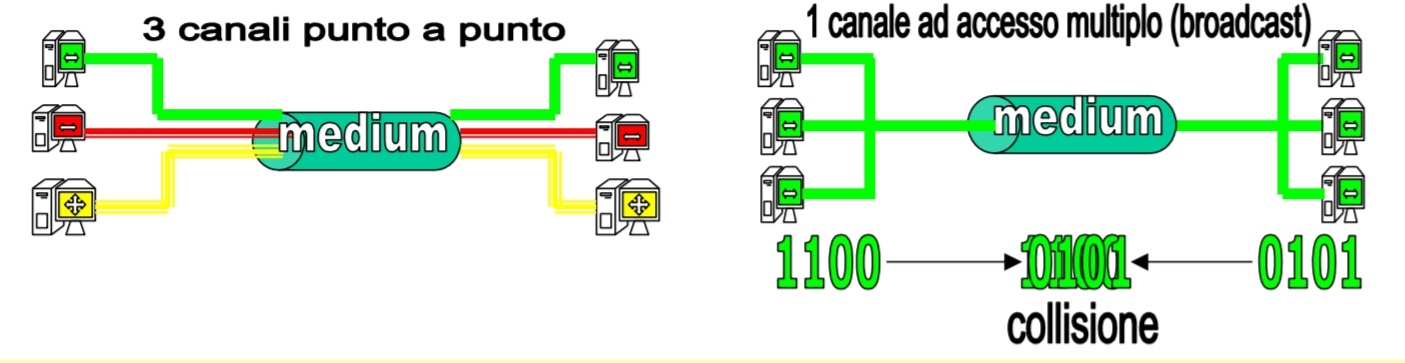
\includegraphics[width=0.8\linewidth]{foto reti di calcolatori/canali di comunicazione.jpg}
\caption{Esempi di canali di comunicazione punto-punto e ad accesso multiplo.}
\end{figure}

\begin{notebox}{}

    Nei canali ad \textbf{accesso multiplo}, i nodi devono gestire l’accesso condiviso al mezzo trasmissivo per evitare collisioni e garantire efficienza.  
    Questi meccanismi vengono regolati da protocolli MAC (Medium Access Control) indirizzi univoci mittente e destinatario.
    
\end{notebox}

\section{Reti di commutazione}

Una \textbf{rete di commutazione} è un tipo di rete nella quale i dati non vengono trasmessi direttamente tra sorgente e destinazione, ma \textbf{instradati attraverso nodi intermedi} (detti \textit{commutatori} o \textit{switch}).  
Ogni nodo ha il compito di ricevere, elaborare e inoltrare le informazioni verso il prossimo nodo fino alla destinazione finale.

\textbf{Obiettivo:} ottimizzare l’uso delle risorse di rete (banda, canali, linee di trasmissione) condividendole tra più comunicazioni.

Esistono due principali modalità di commutazione:
\begin{enumerate}
    \item \textbf{Commutazione di circuito}
    \item \textbf{Commutazione di pacchetto}
\end{enumerate}

\newpage
%-------------------------------------------------
\subsection{Reti a commutazione di circuito }

La \textbf{commutazione di circuito} (Circuit Switching) detta anche \textbf{Circuito riservato}, stabilisce un percorso fisico dedicato tra sorgente e destinazione prima della trasmissione dei dati.

\begin{itemize}
    \item La connessione rimane attiva per tutta la durata della comunicazione.
    \item Le risorse (banda, canale) vengono riservate anche se non utilizzate.
    \item Tipica delle reti telefoniche tradizionali.
\end{itemize}

\begin{figure}[H]
\centering
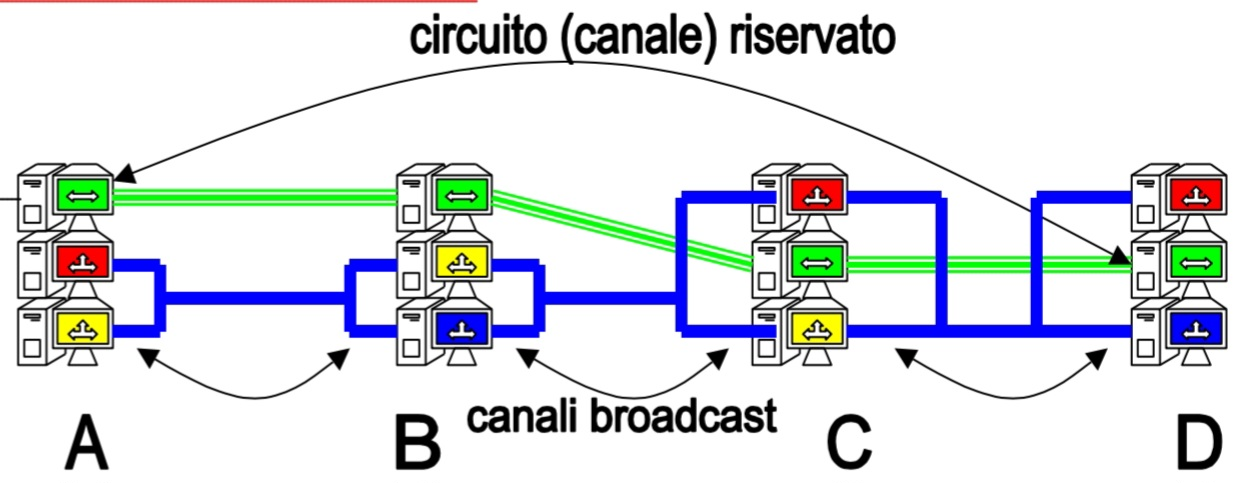
\includegraphics[width=0.8\linewidth]{foto reti di calcolatori/Esempio di rete a commutazione di circuito..jpg}
\caption{Esempio di rete a commutazione di circuito.}
\end{figure}

\textbf{Fasi principali:}
\begin{enumerate}
    \item \textbf{Stabilimento del circuito} — Creazione del percorso dedicato (crea ritardo iniziale di collegamento)
    \item \textbf{Trasferimento dei dati} — Comunicazione continua e ordinata(molto rapida la ricezione)
    \item \textbf{Chiusura del circuito} — Rilascio delle risorse riservate.
\end{enumerate}

\newpage
\subsection{Reti a commutazione di pacchetto}

Nella \textbf{commutazione di pacchetto} (Packet Switching), i dati vengono suddivisi in pacchetti indipendenti, ciascuno dei quali può seguire un percorso diverso nella rete.

\begin{itemize}
    \item Le risorse non vengono prenotate, ma condivise dinamicamente.
    \item Ogni pacchetto contiene informazioni di indirizzamento (mittente e destinatario).
    \item Maggiore ritardo della rete di comunicazione
    \item Si paga per quantità di dati trasmessi (e non per il tempo necessario)
    \item richiede minor numero di risorse di rete, ma meglio utilizzate
    \item È la base di funzionamento delle reti \textbf{Internet (IP)}.
\end{itemize}

\begin{figure}[H]
\centering
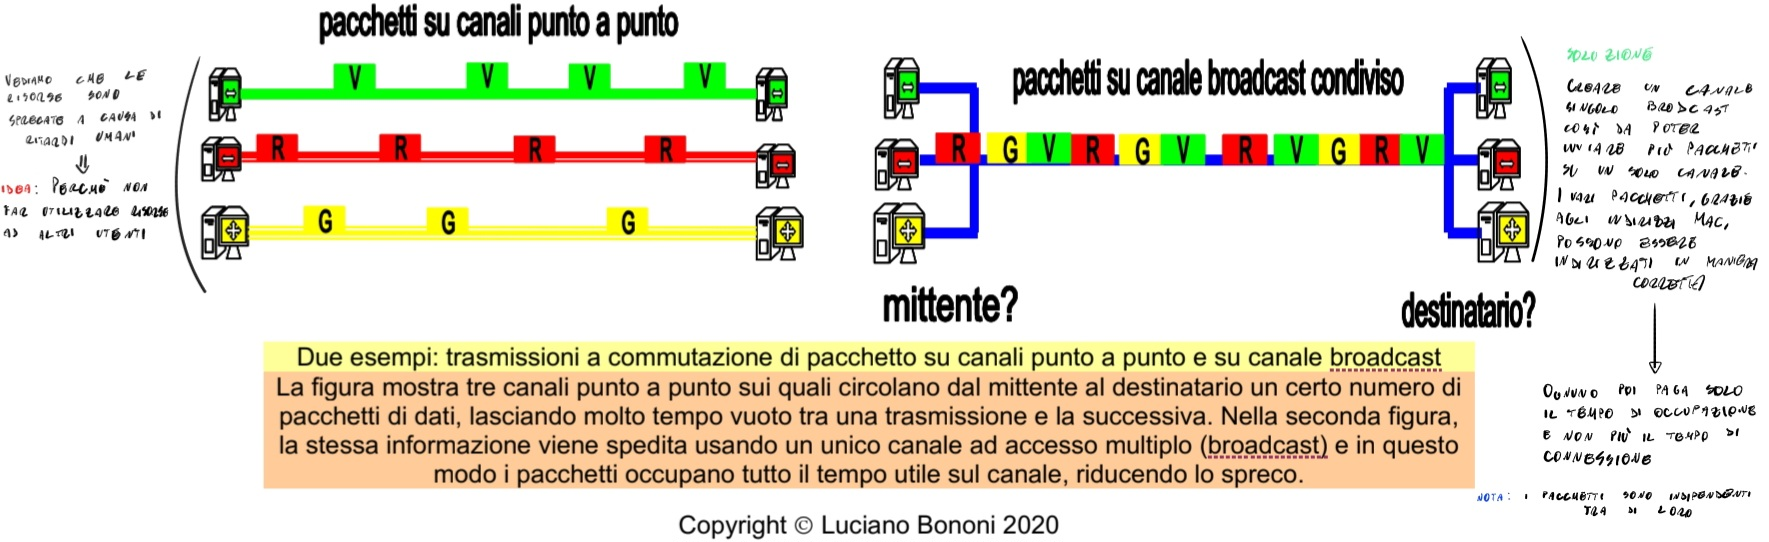
\includegraphics[width=1.1\linewidth]{foto reti di calcolatori/Esempio di rete a commutazione di pacchetto.jpg}
\caption{Esempio di rete a commutazione di pacchetto in cui si crea un singolo canale brodcast in cui inviarepiù pacchetti.}
\end{figure}

\vspace{1em}
\begin{esempiobox}{Confronto tra commutazione di circuito e di pacchetto}
\renewcommand{\arraystretch}{1.3}
\setlength{\tabcolsep}{8pt}
\begin{tabularx}{\linewidth}{>{\bfseries}p{4cm} X X}
\hline
\textbf{Caratteristica} & \textbf{Commutazione di circuito} & \textbf{Commutazione di pacchetto} \\
\hline
Connessione & Necessita di stabilire un circuito dedicato & Non richiede connessione preventiva \\
Uso delle risorse & Risorse riservate e dedicate & Risorse condivise dinamicamente \\
Efficienza & Bassa (tempo di inattività possibile) & Alta (uso ottimale della banda) \\
Ordine dei dati & Dati ricevuti in ordine & I pacchetti possono arrivare disordinati \\
Affidabilità & Elevata, percorso fisso & Variabile, dipende dalla congestione e dai protocolli \\
Latenza & Bassa e costante durante la connessione & Variabile (dipende dal carico della rete) \\
Scalabilità & Limitata (richiede risorse dedicate per ogni connessione) & Elevata (gestisce molti utenti simultaneamente) \\
Qualità del servizio (QoS) & Garantita (banda e percorso riservati) & Non garantita, ma può essere gestita con protocolli specifici (es. DiffServ, MPLS) \\
Gestione del traffico & Semplice, flusso costante,(non richiede instradamento) & Complessa, richiede meccanismi di instradamento e controllo del traffico (si spreca quindi una certa quantità di canale: Overhead)\\
Tipo di tariffazione & Basata sul tempo di connessione & Basata sulla quantità di dati trasmessi \\

Esempi di utilizzo & Rete telefonica tradizionale, ISDN & Internet (rete IP), reti 4G/5G, VoIP \\
\hline
\end{tabularx}
\end{esempiobox}

\begin{notebox}{}
    Da qui in poi verranno usate reti a commutazione di pacchetti
\end{notebox}


\newpage
\section{Servizi orientati alla connessione e non}

Nelle reti a commutazione di pacchetto il servizio di trasmissione dei dati, tra mittente e destinatario ha proprietà determinate dal ruolo dei protocolli di rete utilizzati.

\begin{itemize}
    \item I pacchetti di dati vengono immagazzinati temporaneamente dai dispositivi intermedi lungo il cammino.
    \item Successivamente, i pacchetti vengono inoltrati verso il destinatario finale.
    \item Durante la trasmissione, alcuni pacchetti possono andare perduti per diverse cause (es. congestione o errori di rete).
    \item I pacchetti possono inoltre arrivare a destinazione in un ordine diverso rispetto a quello di invio.
\end{itemize}


\begin{defbox}{Tipologie di servizio}
\begin{itemize}
    \item \textbf{Servizio orientato alla connessione (Connection-Oriented):}\\
    Prima della trasmissione viene stabilita una connessione logica tra mittente e destinatario. 
    I dati vengono inviati in modo ordinato e affidabile.
    Eventuali pacchetti persi verranno ritrasmessi(tramite timer e acknowledgment) .\\
    \textbf{Esempio:} protocollo TCP (Transmission Control Protocol).

    \item \textbf{Servizio non orientato alla connessione (Connectionless):}\\
    Ogni pacchetto è inviato indipendentemente, senza creare una connessione logica. 
    Non è garantito l’ordine o la consegna.\\
    \textbf{Esempio:} lettere di posta ordinaria.
\end{itemize}
\end{defbox}

\begin{figure}[H]
    \centering
    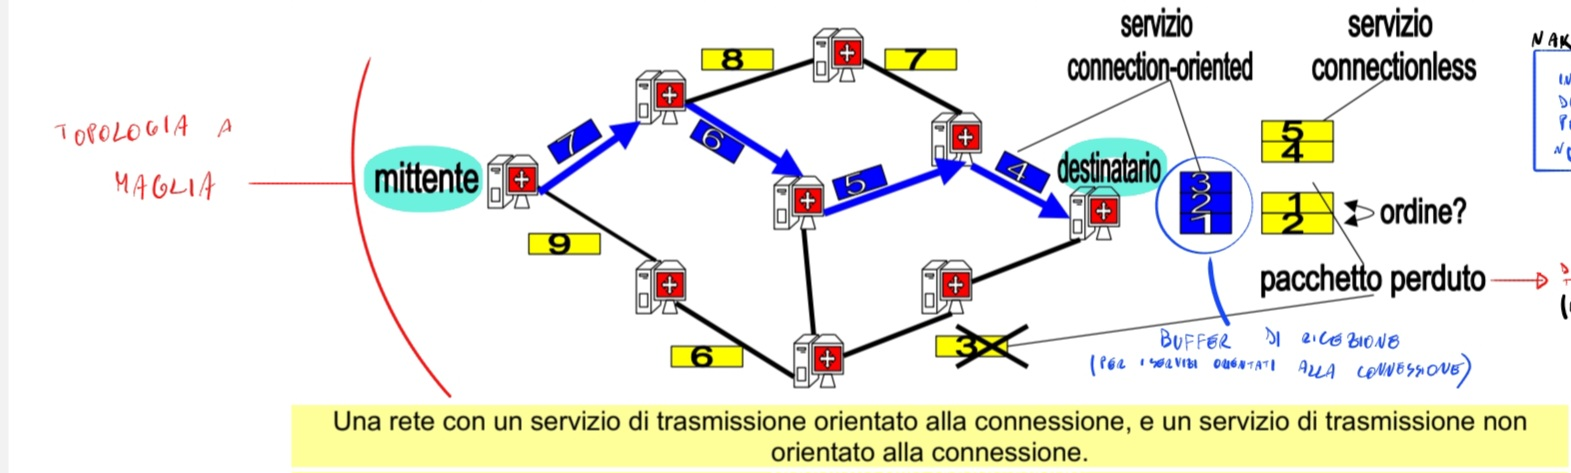
\includegraphics[width=1\linewidth]{foto reti di calcolatori/servizi.jpg}
    \caption{Schema illustrativo dei servizi orientati e non orientati alla connessione.}
   \label{fig:schema_servizi}
\end{figure}



\begin{esempiobox}{Esempio pratico}
Un servizio orientato alla connessione è simile a una telefonata: prima si stabilisce il contatto, poi si parla.  

Un servizio non orientato alla connessione è invece come spedire lettere per posta: ogni messaggio viaggia indipendentemente.
\end{esempiobox}




\subsection{Trasmissione con e senza acknowledgment}

\begin{defbox}{Metodi di trasmissione}
Durante la comunicazione tra \textbf{mittente} e \textbf{destinatario}, possono essere usati due approcci principali:
\begin{itemize}
    \item \textbf{Con acknowledgment (ACK)}: il destinatario invia un messaggio di conferma al mittente per ogni pacchetto ricevuto correttamente.
    \item \textbf{Senza acknowledgment}: il mittente invia i pacchetti senza attendere conferme, assumendo che arrivino correttamente.
\end{itemize}
\end{defbox}

\begin{esempiobox}{Trasmissione con acknowledgment (vedi figura ~\ref{fig:schema_servizi})}
Nel metodo con acknowledgment:
\begin{itemize}
    \item Ogni pacchetto inviato è numerato in modo univoco (\textit{sequence number}).
    \item Il destinatario, alla ricezione, risponde con un \textbf{ACK} che riporta il numero dell’ultimo pacchetto ricevuto correttamente.
    \item Se un pacchetto non viene riconosciuto entro un certo tempo (\textbf{timeout}), il mittente lo ritrasmette. In caso arrivassero duplicati, verrà inviato lo stesso AK in quanto il mittente altrimenti rinvierebbe pacchetti.
\end{itemize}

\textbf{Esempio:}
\begin{itemize}
    \item Il mittente invia i pacchetti numerati 1, 2, 3, 4, 5.
    \item Il destinatario riceve 1, 2, 4, 5 e li memorizza nel buffer, ma il pacchetto 3 va perso.
    \item Invia quindi gli ACK 1, 2, 4, 5 ma il mittente si accorge che \textbf{manca l’ACK 3}.
    \item Scatta il \textbf{timeout} e il pacchetto 3 viene ritrasmesso.
\end{itemize}

Questo metodo garantisce:
\begin{itemize}
    \item Affidabilità;
    \item Ordine corretto di consegna;
    \item Controllo degli errori tramite ritrasmissione.
\end{itemize}
\end{esempiobox}

\begin{notebox}{Trasmissione senza acknowledgment}
Nel metodo senza acknowledgment:
\begin{itemize}
    \item Il mittente non attende conferme dal destinatario;
    \item Non c’è controllo di errori o ritrasmissione;
    \item È più veloce ma meno affidabile.
\end{itemize}

Questo approccio è adatto a \textbf{applicazioni in tempo reale}, dove la perdita di qualche pacchetto è accettabile (es. streaming o chiamate VoIP), ma la latenza deve essere minima.
\end{notebox}

\begin{esempiobox}{Duplicati e loro origine}
I \textbf{pacchetti duplicati} possono verificarsi quando:
\begin{itemize}
    \item il mittente non riceve l’ACK in tempo (per ritardo o perdita dell’ACK stesso);
    \item ritrasmette quindi un pacchetto che in realtà era già arrivato al destinatario.
\end{itemize}

Il destinatario, ricevendo lo stesso pacchetto due volte, può riconoscerlo tramite il numero di sequenza e \textbf{eliminare il duplicato}.
\end{esempiobox}



\vspace{2cm}
\subsection{Il problema dei due generali}


Un concetto fondamentale per comprendere i limiti della comunicazione affidabile in rete è il \textbf{problema dei due generali}.  

Dimostra che, in un sistema dove i messaggi possono essere persi, non è possibile ottenere la certezza assoluta che due entità abbiano raggiunto un accordo condiviso.



\begin{esempiobox}{Descrizione del problema}
Due generali si trovano su due colline opposte e devono coordinare un attacco contro un nemico situato nella valle.  

Possono comunicare solo inviando messaggeri attraverso la valle, ma questi possono essere catturati o uccisi.  
Anche se uno dei generali riceve un messaggio e invia una conferma, l’altro non può sapere con certezza se la conferma è stata ricevuta.  

\textbf{Conclusione:} nessun protocollo può garantire un accordo perfettamente certo in presenza di canali inaffidabili.
\end{esempiobox}

\begin{notebox}{}
Questo paradosso dimostra che in un sistema distribuito, con canale di comunicazione inaffidabile, \textbf{non è possibile garantire accordo perfetto} tra le parti.
\end{notebox}

\subsection*{Risoluzioni pratiche nei protocolli reali}

\begin{itemize}
    \item \textbf{Acknowledgment (ACK):} ogni pacchetto ricevuto correttamente genera un messaggio di conferma.  
    \item \textbf{Timeout e ritrasmissione:} se non arriva conferma entro un certo tempo, il pacchetto viene ritrasmesso.  
    \item \textbf{Numerazione dei pacchetti:} consente di ricostruire l’ordine corretto e individuare duplicati.  
    \item \textbf{Checksum e controllo d’errore:} verifica l’integrità dei dati ricevuti.  
\end{itemize}

\begin{notebox}{}
Questi meccanismi non eliminano l’incertezza logica del problema, ma riducono al minimo la probabilità di errore, ottenendo una comunicazione \textbf{praticamente affidabile}.
\end{notebox}



\newpage
% ============================================================
% SEZIONE: Architettura dei protocolli di rete
% ============================================================
\section{Architettura dei protocolli di rete}

\begin{defbox}{Protocollo di rete}
Un \textbf{protocollo di rete} è un insieme di regole che definiscono come due o più entità comunicano attraverso una rete.  
In particolare, stabilisce:
\begin{itemize}
    \item \textbf{Regole sintattiche}: specificano la \textit{forma} dei dati, cioè i formati dei messaggi, la struttura dei campi e l’ordine in cui devono essere inviati o ricevuti.  
    \item \textbf{Regole semantiche}: definiscono il \textit{significato} e le \textit{procedure operative}, ossia le azioni che ciascuna entità deve compiere in risposta ai messaggi ricevuti (gestione, controllo, risposte, ecc.).  

\end{itemize}

I protocolli garantiscono che dispositivi e sistemi diversi possano \textbf{interoperare} in modo corretto, purché conformi allo stesso standard di comunicazione.
\end{defbox}


\begin{figure}[H]
    \centering
    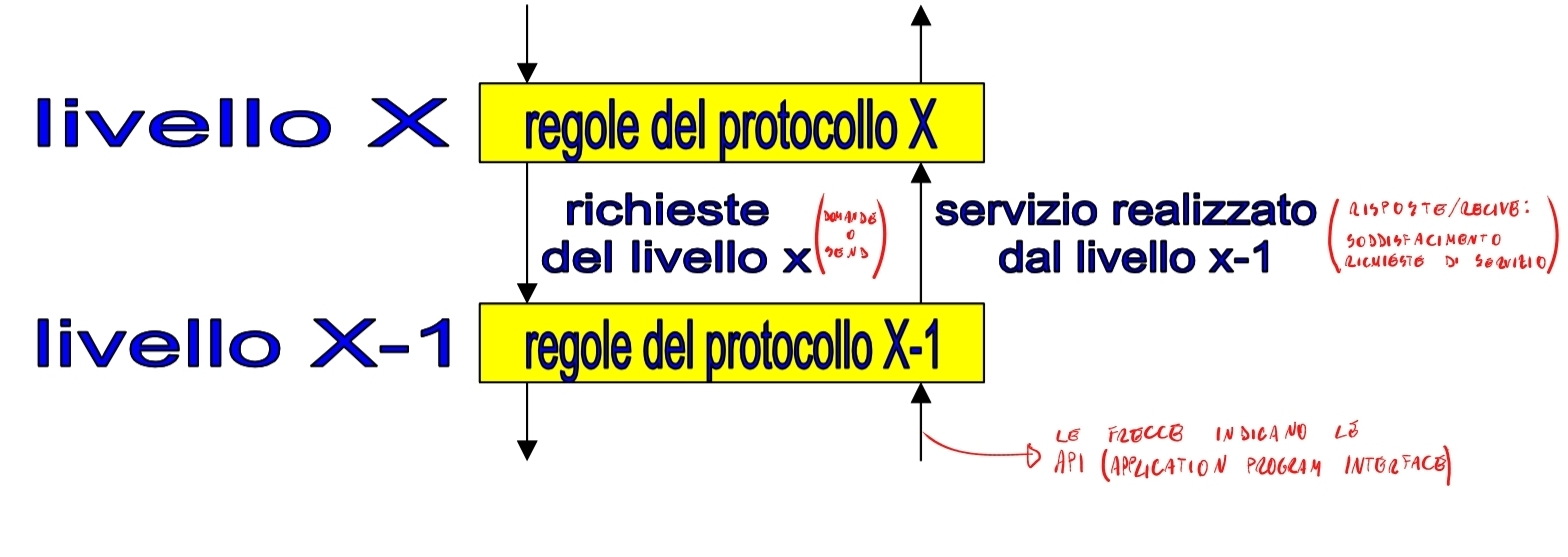
\includegraphics[width=0.95\linewidth]{foto reti di calcolatori/Livelli_protocolli.jpg}
    \caption{Architettura a livelli: idea generale (livello X richiede servizi al livello X-1; regole del protocollo e interfacce).}
\end{figure}

\begin{notebox}{}
Suddividere la comunicazione in livelli (architettura a strati) semplifica la progettazione: ogni livello ha responsabilità ben definite e comunica soltanto con il livello omologo sull'host remoto tramite protocolli e con il livello adiacente locale tramite interfacce di servizio.
\end{notebox}

\subsection*{Perché usare un'architettura a livelli?}
\begin{itemize}
    \item \textbf{Separazione delle responsabilità:} ogni livello affronta un insieme limitato di problemi; 
    \begin{itemize}
        \item I livelli superiori effettuano richieste di servizio al loro livello inferiore
        \item I livelli inferiori forniscono servizi al loro livello superiore
    \end{itemize}
    \item \textbf{Modularità:} è possibile cambiare o aggiornare un livello senza riscrivere gli altri.
    \item \textbf{Standardizzazione:} facilita compatibilità e interoperabilità.
    \item \textbf{Astrazione:} i livelli superiori non devono conoscere i dettagli implementativi di quelli inferiori.
\end{itemize}


\subsection{Standard ISO/OSI RM (Open System Interconnection Reference Model)}

Lo \textbf{Standard ISO/OSI RM}  definisce un’architettura a \textbf{sette livelli} che suddivide le funzioni di comunicazione in moduli distinti, ognuno con un ruolo specifico.  

Ogni livello fornisce servizi al livello superiore e utilizza i servizi offerti da quello inferiore.  

Nella pila dei protocolli di rete, si distinguono due istanze:

una nel nodo mittente e una nel nodo destinatario, ognuna composta dagli stessi sette livelli, numerati dall’alto verso il basso (7 → 1).  

Ogni protocollo dello stesso colore è come se comunicasse direttamente con quello adiacenti 

\begin{figure}[H]
    \centering
    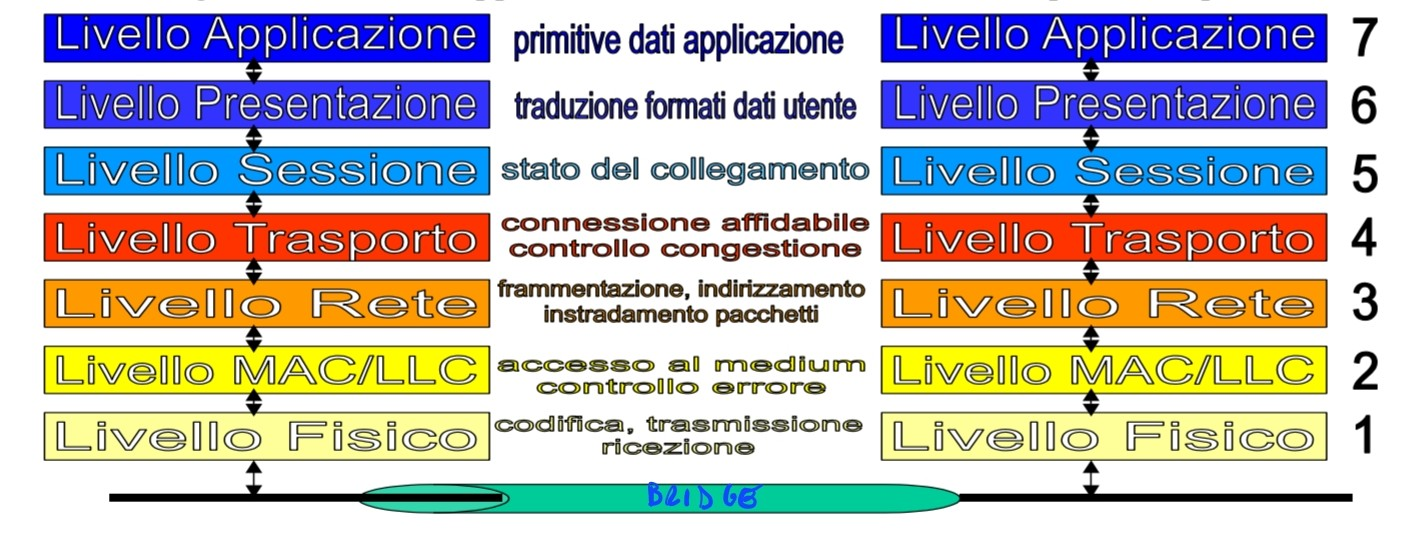
\includegraphics[width=0.95\linewidth]{foto reti di calcolatori/ISO.jpg}
    \caption{La pila di livelli dei protocolli di rete dello standard ISO/OSI.
    Mostrate due istanze, una per il nodo mittente e una per il nodo destinatario, dei sette livelli di protocolli di rete dello Standard.}
\end{figure}

\vspace{1cm}
\begin{itemize}
         \item \textbf{Livello 7 – Applicazione:}  
    \begin{itemize}
        \item livello in cui sono in esecuzione i protocolli che permettono all'utente di comunicare(applicazione browser sta sopra a questo livello)
        \item Fornisce i \textbf{servizi di comunicazione direttamente alle applicazioni utente} (client/server).
        \item Gestisce la trasmissione e la ricezione dei dati applicativi, come posta elettronica, web e trasferimento di file.
        \item Offre interfacce e primitive(standard) di comunicazione per i programmi utente.
        \item \textit{Esempi di protocolli:} HTTP(modo che ha il browser per chiedere al livello 7 richiesta dell pagina web), FTP, SMTP, POP3, IMAP.
        \item \textit{Dispositivi tipici:} computer, server, smartphone.
    \end{itemize}

    \item \textbf{Livello 6 (obsoleto)– Presentazione:}  
    \begin{itemize}
        \item Si occupa della \textbf{rappresentazione dei dati} per garantire compatibilità tra sistemi diversi.
        \item Gestisce la \textbf{codifica dei caratteri} (es. ASCII, UTF-8), la \textbf{compressione} e la \textbf{cifratura/decifratura}.
        \item Risolve eventuali differenze(dovute alla traduzione) di formato e struttura dei dati (esempio little-endian in big-endian).
        \item \textit{Esempi di protocolli:} SSL/TLS, formati MIME, JPEG, MP3.
    \end{itemize}

    \item \textbf{Livello 5 (obsoleto) – Sessione:}  
    \begin{itemize}
        \item Mantiene e controlla la sessione di comunicazione tra mittente e destinatario.
        \item Gestisce l’apertura, la chiusura e la sincronizzazione delle sessioni di comunicazione.
        \item Permette il \textbf{ripristino} (recovery) di una sessione in caso di interruzioni. Tale ripristino viene salvato proprio in questo livello per far si che vengano riprese le trasmissioni da dove erano state interrotte.
        \item \textit{Esempi di protocolli:} NetBIOS, RPC, protocolli di gestione sessione nelle API di rete.
    \end{itemize}

    \item \textbf{Livello 4 – Trasporto:}  
    \begin{itemize}
        \item Fornisce un servizio di comunicazione \textbf{processo-a-processo}.
        \item Può essere \textbf{affidabile} (con controllo errori e ritrasmissione) o \textbf{non affidabile}.
        \item  Ci si preoccupa anche del ritmo ideale di invio dei pacchetti nella rete
        \item Implementa:
        \begin{enumerate}
            \item controllo di flusso tra mittente e destinatario (al fine di accelerare o rallentare l'invio di pacchetti);
            \item ritrasmissione dei pacchetti persi (con acknowledgment);
            \item controllo della congestione della rete (per far si che il buffer del router non si riempa e non vengano persi) 
        \end{enumerate}
        \item L’unità di dati è il \textbf{segmento}, rappresentato come una \textbf{\textcolor{red}{busta rossa}}.
        \item \textit{Esempi di protocolli:} TCP connectio-oriented(affidabile, orientato alla connessione), UDP Connectionless(non affidabile, senza connessione).
    \end{itemize}

    \item \textbf{Livello 3 – Rete:}  
    \begin{itemize}
    \item Gestisce l’\textbf{instradamento} (\textit{routing}) dei pacchetti e l’\textbf{indirizzamento logico} tramite indirizzi \textbf{IP}\footnote{Gli indirizzi IP (Internet Protocol) identificano in modo univoco ogni dispositivo connesso a una rete, permettendo l'instradamento dei pacchetti verso la destinazione corretta. 
    Sono ben strutturati e seguono ordine gerarchico: nome rete destinatario - nome host.}
    
    \item È il livello che \textbf{unifica tutte le reti locali} collegandole tra loro tramite i \textbf{router}, che andrà ad applicare il protocollo 3.
    Questo router viene usato come rappresentatnte che prende i pacchetti e guarda quale si la rete del destinatario(a seguire l'host giusto).
    \item Determina il percorso ottimale che un pacchetto deve seguire dalla sorgente alla destinazione.
    
    \item Si occupa anche della \textbf{frammentazione dei pacchetti}, ma \textbf{solo in IPv4} (in IPv6 la frammentazione non è più gestita dal router, ma dall’host sorgente).
    
    \item L’unità di dati è il \textbf{pacchetto}, rappresentato come una \textbf{\textcolor{orange}{busta arancione}}.
    \item \textit{Esempi di protocolli:} IP, ICMP, OSPF, BGP.
    \item \textit{Dispositivi tipici:} router.
    \end{itemize}
  
    \newpage
        \item \textbf{Livello 2 – Collegamento Dati (MAC/LLC):} 
        è formato da 2 sottolivelli che risolvono problemi distinti:
        \begin{itemize}
            \item \textbf{MAC}
            \begin{enumerate}
                \item costruisce il formato sintattico del pacchetto (com è composta la sequenza di bit)
                \item  L’unità di dati è il \textbf{frame}, rappresentato come una \textbf{\textcolor{yellow}{busta gialla}}, che contiene: 
                
                > Mac adress (mittente e destinatario, ovvero quale scheda di rete è destinataria/mittente del frame trasmesso?),
                
                > dati e CRC (per il controllo di errori)

                \item \textbf{Trasmissione:} gestisce l’accesso al canale condiviso (\textbf{arbitraggio}), decidendo chi trasmette e quando, per evitare collisioni.  
                Ogni frame viene inviato sul mezzo trasmissivo e ricevuto da tutte le schede di rete, ma solo quella con l’indirizzo MAC corrispondente lo accetta.

                \item \textbf{Ricezione:} verificare se il frame ricevuto è destinato al proprio indirizzo MAC; in caso affermativo, viene accettato e passato ai livelli superiori.
            \end{enumerate}
            
            \item \textbf{LLC (logical link control)}
            permette di capire se il frame è corretto ed in caso positivo manda Acknoledgment.

            Per capire se ci sono errori viene attivato un timer che farà rinviare il frame in caso non ricevesse Acknoledgment.
            \end{itemize}
             
        \textit{Esempi di tecnologie:} Ethernet, Wi-Fi.  
        \textit{Dispositivi tipici:} switch,bridge schede di rete (NIC).
    
        \item \textbf{Livello 1 – Fisico:} 
        
        Si occupa della trasmissione dei \textbf{bit} grezzi sul mezzo fisico (rame, fibra, radio).  
    
        in particolare si occupa di \textbf{codifica,trasmissione e ricezione} dei segnali bit (da bit a segnali elettrici e viceversa)
\end{itemize}


\begin{notebox}{Osservazione}
Nella pratica, le reti reali non seguono rigidamente lo schema ISO/OSI, ma si ispirano ad esso.  
Il modello OSI rimane un riferimento teorico utile per comprendere la separazione dei compiti nei protocolli.  
L’architettura \textbf{TCP/IP}, derivata e semplificata, è quella effettivamente adottata nelle reti moderne, come Internet.
\end{notebox}














\chapter{Conversione tra basi numeriche}

\section{Funzione valore (da base \(B\) a base 10)}

Sia un numero rappresentato in base \(B\) come:
\[
(b_{n-1} b_{n-2} \ldots b_1 b_0)_B
\]

La sua rappresentazione in base 10 è data dalla \textbf{funzione valore}:
\[
D = \sum_{i=0}^{n-1} b_i \cdot B^i
\]

\subsubsection*{Esempio 1}
Convertire \( (1\,2\,2)_3 \) in base 10:
\[
1 \cdot 3^2 + 2 \cdot 3^1 + 2 \cdot 3^0 = 9 + 6 + 2 = \boxed{17_{10}}
\]

\subsubsection*{Esempio 2}
Convertire \( (2\,4\,1\,1\,3)_5 \) in base 10:
\[
2 \cdot 5^4 + 4 \cdot 5^3 + 1 \cdot 5^2 + 1 \cdot 5^1 + 3 \cdot 5^0 = 1250 + 500 + 25 + 5 + 3 = \boxed{1783_{10}}
\]

\newpage
%-------------------------------------------------
\section{Algoritmo di divisione (da base 10 a base \(B\))}

Per convertire un numero decimale \(D\) in base \(B\), si divide successivamente il numero per \(B\), annotando i resti.  
I resti letti dal basso verso l’alto formano il numero nella nuova base.

\subsubsection*{Esempio: \(1783_{10} \rightarrow \) base 7}
\[
\begin{array}{rcl}
1783 \div 7 &=& 254 \quad \text{con resto } \boxed{5} \\
254 \div 7 &=& 36 \quad \text{con resto } \boxed{2} \\
36 \div 7 &=& 5 \quad \text{con resto } \boxed{1} \\
5 \div 7 &=& 0 \quad \text{con resto } \boxed{5}
\end{array}
\]
\[
\Rightarrow (1783)_{10} = \boxed{5\,1\,2\,5}_7
\]

%-------------------------------------------------
\subsection{Trucco galattico: Conversione decimale $\rightarrow$ binario}

\textbf{Idea:}  
Per convertire un numero decimale in binario senza fare tutte le divisioni, si può usare il \textbf{trucco galattico ;)}:  
si scompone il numero nelle potenze di 2 più grandi possibili e si segna un \texttt{1} nelle posizioni corrispondenti.

\begin{enumerate}
    \item Si individua la massima potenza di 2 minore o uguale al numero.
    \item Si sottrae tale potenza e si ripete il processo con il resto.
    \item Ogni potenza di 2 usata corrisponde a un bit impostato a 1; le altre a 0.
\end{enumerate}

\subsubsection*{Esempio: \(218_{10} \rightarrow \) base 2}
\begin{align*}
218 - 2^7 &= 90 \quad (2^7 = 128) \\
90 - 2^6 &= 26 \quad (2^6 = 64) \\
26 - 2^4 &= 10 \quad (2^4 = 16) \\
10 - 2^3 &= 2 \quad (2^3 = 8) \\
2 - 2^1 &= 0 \quad (2^1 = 2)
\end{align*}

Le potenze usate sono: \(2^7, 2^6, 2^4, 2^3, 2^1\).  
Quindi, scrivendo un bit per ogni potenza da \(2^7\) a \(2^0\):

\[
\Rightarrow \boxed{11011010}_2 \quad \text{(8 bit)}
\]

\begin{notebox}{\textbf{Potenze di 2 fino a \(2^{25}\):}}

\begin{align*}
2^0 &= 1 &\quad 2^9  &= 512 &\quad 2^{18} &= 262.144 \\
2^1 &= 2 &\quad 2^{10} &= 1.024 &\quad 2^{19} &= 524.288 \\
2^2 &= 4 &\quad 2^{11} &= 2.048 &\quad 2^{20} &= 1.048.576 \\
2^3 &= 8 &\quad 2^{12} &= 4.096 &\quad 2^{21} &= 2.097.152 \\
2^4 &= 16 &\quad 2^{13} &= 8.192 &\quad 2^{22} &= 4.194.304 \\
2^5 &= 32 &\quad 2^{14} &= 16.384 &\quad 2^{23} &= 8.388.608 \\
2^6 &= 64 &\quad 2^{15} &= 32.768 &\quad 2^{24} &= 16.777.216 \\
2^7 &= 128 &\quad 2^{16} &= 65.536 &\quad 2^{25} &= 33.554.432 \\
2^8 &= 256 &\quad 2^{17} &= 131.072 &&
\end{align*}

\end{notebox}




\newpage
\section{Conversione tra basi binaria, ottale ed esadecimale}

Le basi \textbf{2}, \textbf{8} e \textbf{16} sono strettamente correlate perché sono tutte potenze di 2:
\[
8 = 2^3 \quad \text{e} \quad 16 = 2^4
\]
Ciò permette conversioni \textbf{dirette e immediate} tra queste basi, senza passare per la base 10.

---

\subsection*{Conversione Binario $\leftrightarrow$ Ottale}

Per convertire un numero binario in ottale:
\begin{enumerate}
    \item Si raggruppano le cifre binarie in gruppi di \textbf{3 bit} (a partire da destra).
    \item Ogni gruppo viene convertito nel corrispondente valore ottale.
\end{enumerate}

Esempio:
\[
(101110)_2 = (101)(110)_2 = (5)(6)_8 = \boxed{56_8}
\]

\begin{center}
\renewcommand{\arraystretch}{1.2}
\setlength{\tabcolsep}{10pt}
\begin{tabular}{|c|c|}
\hline
\textbf{Binario (3 bit)} & \textbf{Ottale} \\
\hline
000 & 0 \\
001 & 1 \\
010 & 2 \\
011 & 3 \\
100 & 4 \\
101 & 5 \\
110 & 6 \\
111 & 7 \\
\hline
\end{tabular}
\captionof{table}{Tabella di conversione binario $\leftrightarrow$ ottale}
\end{center}


\subsection*{Conversione Binario $\leftrightarrow$ Esadecimale}

Per convertire un numero binario in esadecimale:
\begin{enumerate}
    \item Si raggruppano le cifre binarie in gruppi di \textbf{4 bit} (a partire da destra).
    \item Ogni gruppo viene tradotto nella corrispondente cifra esadecimale (0–9, A–F).
\end{enumerate}

Esempio:
\[
(110101111001)_2 = (1101)(0111)(1001)_2 = (D)(7)(9)_{16} = \boxed{D79_{16}}
\]

\begin{center}
\renewcommand{\arraystretch}{1.2}
\setlength{\tabcolsep}{8pt}
\begin{tabular}{|c|c||c|c|}
\hline
\textbf{Binario (4 bit)} & \textbf{Hex} & \textbf{Binario (4 bit)} & \textbf{Hex} \\
\hline
0000 & 0 & 1000 & 8 \\
0001 & 1 & 1001 & 9 \\
0010 & 2 & 1010 & A \\
0011 & 3 & 1011 & B \\
0100 & 4 & 1100 & C \\
0101 & 5 & 1101 & D \\
0110 & 6 & 1110 & E \\
0111 & 7 & 1111 & F \\
\hline
\end{tabular}
\captionof{table}{Tabella di conversione binario $\leftrightarrow$ esadecimale}
\end{center}


\newpage
\section{Tabella completa dei numeri da 0 a 255 in Binario (8 bit)}

In questa sezione sono riportati tutti i valori decimali compresi tra 0 e 255 con la relativa rappresentazione binaria a 8 bit. In \textbf{\textcolor{red}{rosso}} sono evidenziati i valori fondamentali utilizzati per il calcolo delle \textbf{Subnet Mask}.

{ % Inizio gruppo locale per non alterare il resto del documento
\renewcommand{\arraystretch}{0.95} % Riduce l'altezza delle righe (ignora l'1.2 del preambolo)
\scriptsize % Font più piccolo per far stare 64 righe in una pagina
\setlength{\tabcolsep}{4pt} % Riduce leggermente lo spazio orizzontale tra le celle

\begin{center}
\begin{tabular}{|c|c||c|c||c|c||c|c|}
\hline
\textbf{Dec} & \textbf{Bin} & \textbf{Dec} & \textbf{Bin} & \textbf{Dec} & \textbf{Bin} & \textbf{Dec} & \textbf{Bin} \\ 
\hline

\textbf{\textcolor{red}{0}} & \textbf{\textcolor{red}{00000000}} & 64 & 01000000 & \textbf{\textcolor{red}{128}} & \textbf{\textcolor{red}{10000000}} & \textbf{\textcolor{red}{192}} & \textbf{\textcolor{red}{11000000}} \\
1 & 00000001 & 65 & 01000001 & 129 & 10000001 & 193 & 11000001 \\
2 & 00000010 & 66 & 01000010 & 130 & 10000010 & 194 & 11000010 \\
3 & 00000011 & 67 & 01000011 & 131 & 10000011 & 195 & 11000011 \\
4 & 00000100 & 68 & 01000100 & 132 & 10000100 & 196 & 11000100 \\
5 & 00000101 & 69 & 01000101 & 133 & 10000101 & 197 & 11000101 \\
6 & 00000110 & 70 & 01000110 & 134 & 10000110 & 198 & 11000110 \\
7 & 00000111 & 71 & 01000111 & 135 & 10000111 & 199 & 11000111 \\
8 & 00001000 & 72 & 01001000 & 136 & 10001000 & 200 & 11001000 \\
9 & 00001001 & 73 & 01001001 & 137 & 10001001 & 201 & 11001001 \\
10 & 00001010 & 74 & 01001010 & 138 & 10001010 & 202 & 11001010 \\
11 & 00001011 & 75 & 01001011 & 139 & 10001011 & 203 & 11001011 \\
12 & 00001100 & 76 & 01001100 & 140 & 10001100 & 204 & 11001100 \\
13 & 00001101 & 77 & 01001101 & 141 & 10001101 & 205 & 11001101 \\
14 & 00001110 & 78 & 01001110 & 142 & 10001110 & 206 & 11001110 \\
15 & 00001111 & 79 & 01001111 & 143 & 10001111 & 207 & 11001111 \\
16 & 00010000 & 80 & 01010000 & 144 & 10010000 & 208 & 11010000 \\
17 & 00010001 & 81 & 01010001 & 145 & 10010001 & 209 & 11010001 \\
18 & 00010010 & 82 & 01010010 & 146 & 10010010 & 210 & 11010010 \\
19 & 00010011 & 83 & 01010011 & 147 & 10010011 & 211 & 11010011 \\
20 & 00010100 & 84 & 01010100 & 148 & 10010100 & 212 & 11010100 \\
21 & 00010101 & 85 & 01010101 & 149 & 10010101 & 213 & 11010101 \\
22 & 00010110 & 86 & 01010110 & 150 & 10010110 & 214 & 11010110 \\
23 & 00010111 & 87 & 01010111 & 151 & 10010111 & 215 & 11010111 \\
24 & 00011000 & 88 & 01011000 & 152 & 10011000 & 216 & 11011000 \\
25 & 00011001 & 89 & 01011001 & 153 & 10011001 & 217 & 11011001 \\
26 & 00011010 & 90 & 01011010 & 154 & 10011010 & 218 & 11011010 \\
27 & 00011011 & 91 & 01011011 & 155 & 10011011 & 219 & 11011011 \\
28 & 00011100 & 92 & 01011100 & 156 & 10011100 & 220 & 11011100 \\
29 & 00011101 & 93 & 01011101 & 157 & 10011101 & 221 & 11011101 \\
30 & 00011110 & 94 & 01011110 & 158 & 10011110 & 222 & 11011110 \\
31 & 00011111 & 95 & 01011111 & 159 & 10011111 & 223 & 11011111 \\
32 & 00100000 & 96 & 01100000 & 160 & 10100000 & \textbf{\textcolor{red}{224}} & \textbf{\textcolor{red}{11100000}} \\
33 & 00100001 & 97 & 01100001 & 161 & 10100001 & 225 & 11100001 \\
34 & 00100010 & 98 & 01100010 & 162 & 10100010 & 226 & 11100010 \\
35 & 00100011 & 99 & 01100011 & 163 & 10100011 & 227 & 11100011 \\
36 & 00100100 & 100 & 01100100 & 164 & 10100100 & 228 & 11100100 \\
37 & 00100101 & 101 & 01100101 & 165 & 10100101 & 229 & 11100101 \\
38 & 00100110 & 102 & 01100110 & 166 & 10100110 & 230 & 11100110 \\
39 & 00100111 & 103 & 01100111 & 167 & 10100111 & 231 & 11100111 \\
40 & 00101000 & 104 & 01101000 & 168 & 10101000 & 232 & 11101000 \\
41 & 00101001 & 105 & 01101001 & 169 & 10101001 & 233 & 11101001 \\
42 & 00101010 & 106 & 01101010 & 170 & 10101010 & 234 & 11101010 \\
43 & 00101011 & 107 & 01101011 & 171 & 10101011 & 235 & 11101011 \\
44 & 00101100 & 108 & 01101100 & 172 & 10101100 & 236 & 11101100 \\
45 & 00101101 & 109 & 01101101 & 173 & 10101101 & 237 & 11101101 \\
46 & 00101110 & 110 & 01101110 & 174 & 10101110 & 238 & 11101110 \\
47 & 00101111 & 111 & 01101111 & 175 & 10101111 & 239 & 11101111 \\
48 & 00110000 & 112 & 01110000 & 176 & 10110000 & \textbf{\textcolor{red}{240}} & \textbf{\textcolor{red}{11110000}} \\
49 & 00110001 & 113 & 01110001 & 177 & 10110001 & 241 & 11110001 \\
50 & 00110010 & 114 & 01110010 & 178 & 10110010 & 242 & 11110010 \\
51 & 00110011 & 115 & 01110011 & 179 & 10110011 & 243 & 11110011 \\
52 & 00110100 & 116 & 01110100 & 180 & 10110100 & 244 & 11110100 \\
53 & 00110101 & 117 & 01110101 & 181 & 10110101 & 245 & 11110101 \\
54 & 00110110 & 118 & 01110110 & 182 & 10110110 & 246 & 11110110 \\
55 & 00110111 & 119 & 01110111 & 183 & 10110111 & 247 & 11110111 \\
56 & 00111000 & 120 & 01111000 & 184 & 10111000 & \textbf{\textcolor{red}{248}} & \textbf{\textcolor{red}{11111000}} \\
57 & 00111001 & 121 & 01111001 & 185 & 10111001 & 249 & 11111001 \\
58 & 00111010 & 122 & 01111010 & 186 & 10111010 & 250 & 11111010 \\
59 & 00111011 & 123 & 01111011 & 187 & 10111011 & 251 & 11111011 \\
60 & 00111100 & 124 & 01111100 & 188 & 10111100 & \textbf{\textcolor{red}{252}} & \textbf{\textcolor{red}{11111100}} \\
61 & 00111101 & 125 & 01111101 & 189 & 10111101 & 253 & 11111101 \\
62 & 00111110 & 126 & 01111110 & 190 & 10111110 & \textbf{\textcolor{red}{254}} & \textbf{\textcolor{red}{11111110}} \\
63 & 00111111 & 127 & 01111111 & 191 & 10111111 & \textbf{\textcolor{red}{255}} & \textbf{\textcolor{red}{11111111}} \\ 
\hline
\end{tabular}
\end{center}
} % Fine gruppo locale

\vspace{0.5cm} % Spazio aggiuntivo prima del box
\begin{notebox}{Valori fondamentali delle Subnet Mask}
Osservando i numeri evidenziati in \textbf{\textcolor{red}{rosso}}, puoi notare i valori critici utilizzati per il calcolo delle sottomoreti (Subnetting). I valori: \\
\textbf{128, 192, 224, 240, 248, 252, 254, 255} \\
(oltre allo zero) sono gli unici decimali possibili all'interno di una maschera di rete corretta, in quanto corrispondono all'accensione progressiva dei bit da sinistra verso destra.
\end{notebox}


\end{document}
